\documentclass[10pt]{article}
 
\usepackage[margin=1in]{geometry} 
\usepackage{amsmath,amsthm,amssymb, graphicx, multicol, array, minted, listings}
\usepackage{caption, subcaption}
 
\newcommand{\N}{\mathbb{N}}
\newcommand{\Z}{\mathbb{Z}}
\newcommand{\R}{\mathbb{R}}
\newcommand{\C}{\mathbb{C}}
\newcommand{\Q}{\mathbb{Q}}

\newenvironment{problem}[2][Problem]{\begin{trivlist}
\item[\hskip \labelsep {\bfseries #1}\hskip \labelsep {\bfseries #2.}]}{\end{trivlist}}

\begin{document}
Git log file:
\VerbatimInput{log.txt}
\newpage
\title{Lab 3 - Numerical Solution of Ordinary Differential Equations}
\author{Sebastien Abadi\\
Ph20}
\maketitle
 
\begin{problem}{1} 
The explicit Euler's method was used to model a spring's position and velocity for some period of time. For simplicity, that spring was assumed to have $\frac{k}{m}=1$. In Figure 1, we see the positions and velocities of a spring that began with position of -1 and a velocity of 1 over the course of ten oscillations.
\begin{figure}[h]
\centering
\begin{subfigure}{.45\textwidth}
  \centering
  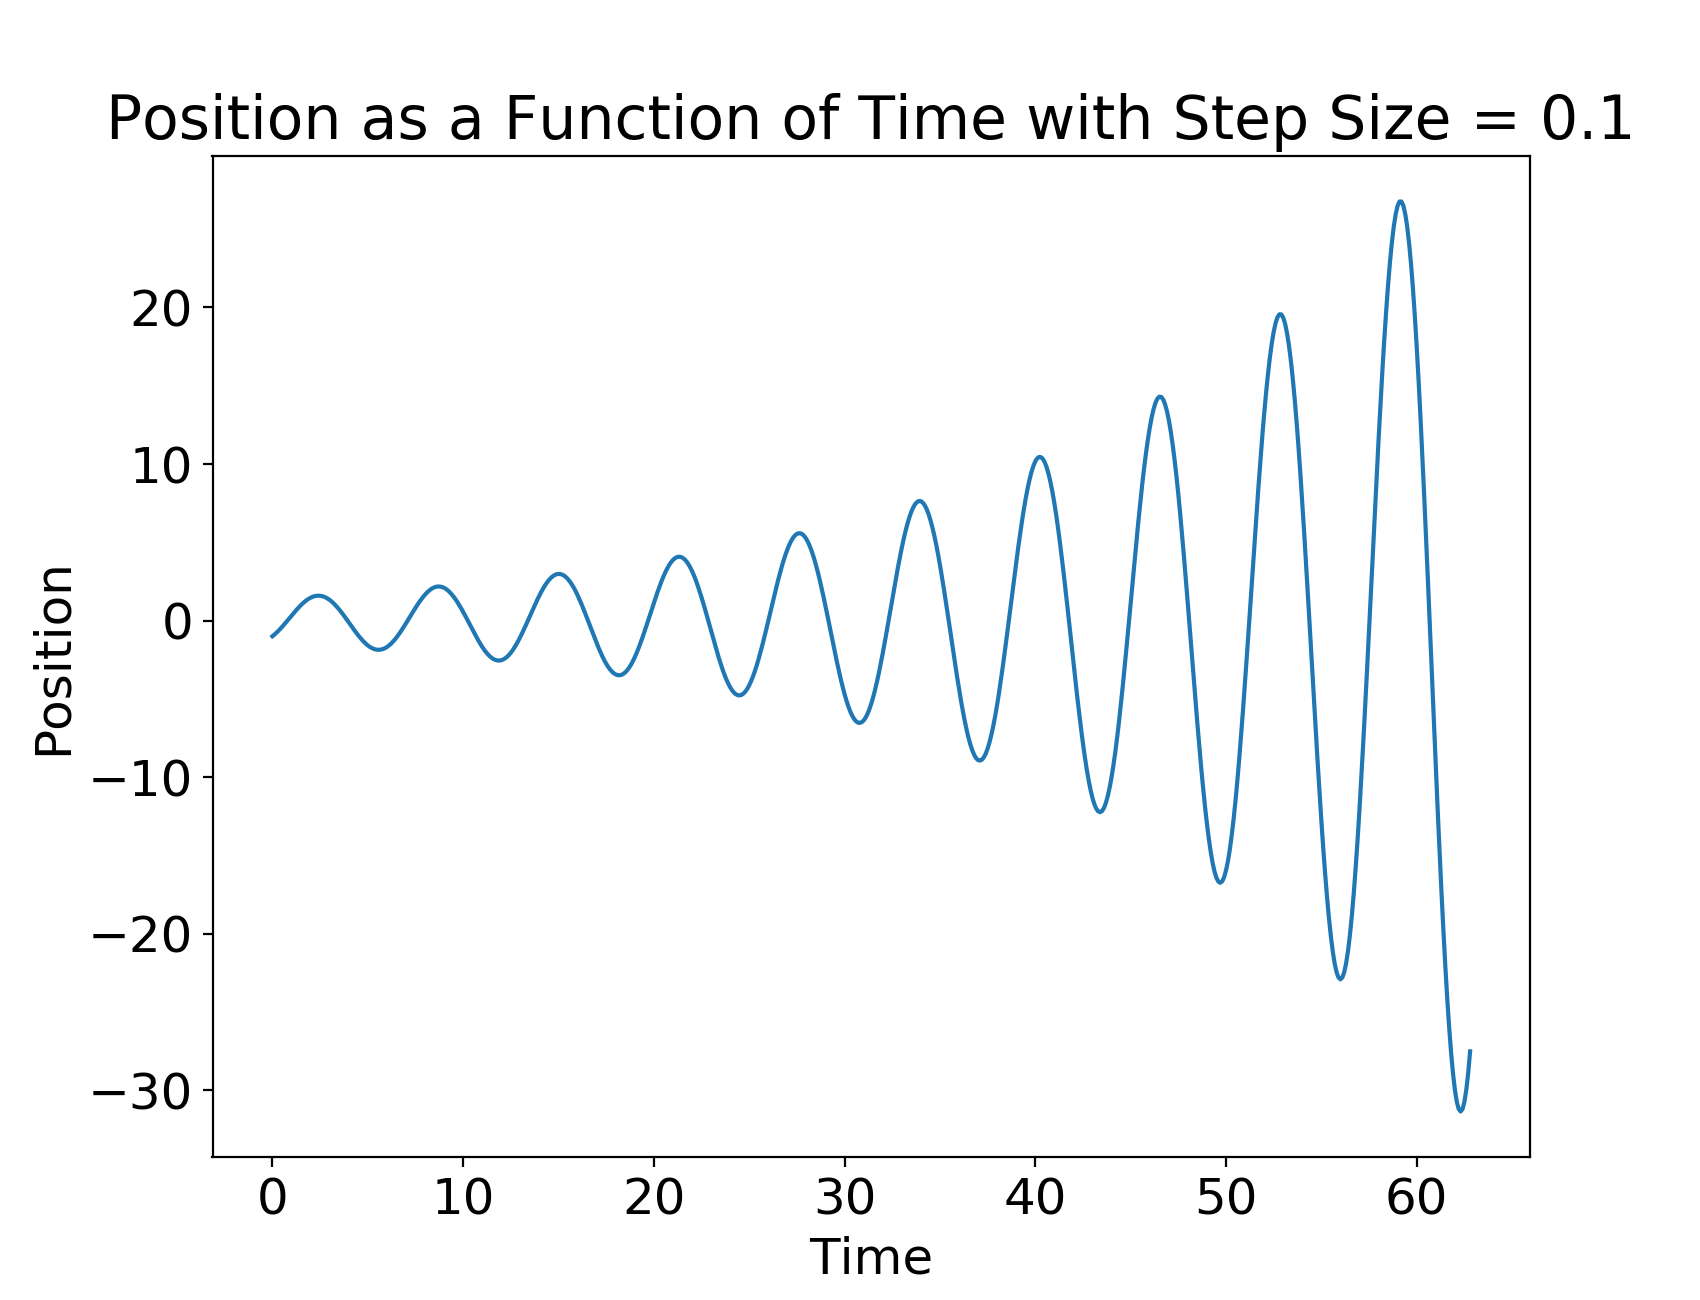
\includegraphics[width=1\linewidth]{PosExp.png}
\end{subfigure}%
\begin{subfigure}{.45\textwidth}
  \centering
  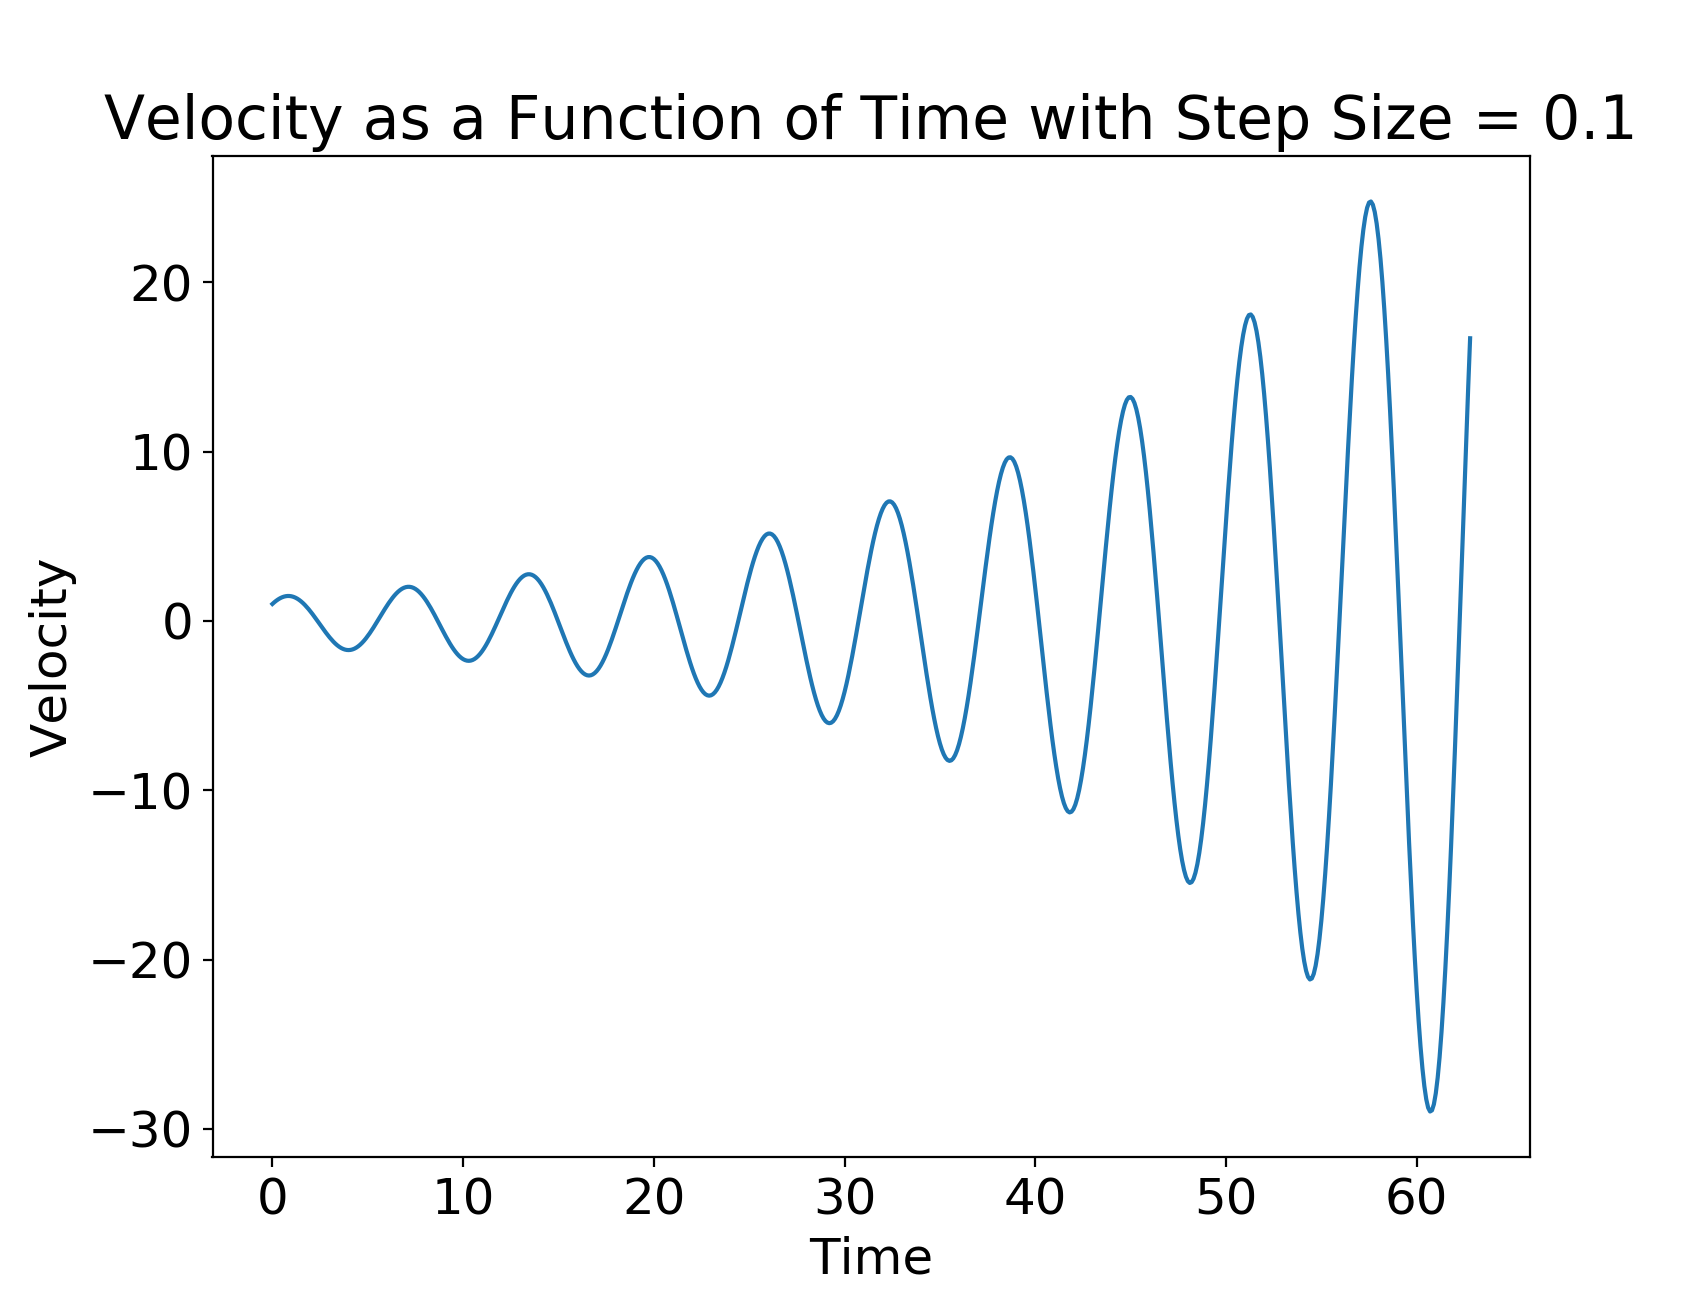
\includegraphics[width=1\linewidth]{VelExp.png}
\end{subfigure}
\caption{Position and Velocity as a Function of Time as Approximated Using the Explicit Euler's Method}
\end{figure}

Note that the peaks of position and velocity are increasing, but that in an ideal spring, energy is conserved so these peaks would be expected to remain at a constant height. Also note that the rate at which the peaks increase appears to itself be increasing, which is consistent with the idea that the error in an approximation at a particular time stems not just from the latest step taken, but also from the error that has accumulated in prior steps.

\end{problem}

\begin{problem}{2}
We will now analytically solve for the position and velocity of a spring with $\frac{k}{m}=1$ as a function of time. By Newton's second law of motion and by Hooke's law $F=ma=-kx$. Thus, $\frac{d^2x}{dt^2}=x$. Observe that a family of solutions satisfying this differential equation is $x = C_1 \cos(\pm t+C_2)$. Then, notice that in the physical system of the spring $C_1$ correspond to maximum displacement, the $\pm$ corresponds to its initial direction of motion, and $-C_2$ corresponds to where in a cycle the spring is at $t=0$. 

We will now find the particular values of these parameters from a given the initial position $x_i$ and velocity $v_i$. First note that we can find the energy $E$ of the spring system to be $\frac{1}{2}kx_i^2 + \frac{1}{2}mv_i^2$.
Note that the spring will attain maximum displacement when the velocity is zero, and that at that time, by conservation of energy the energy of the system will be the same as it was initially. Thus, $\frac{1}{2}kx_{max}^2= \frac{1}{2}kx_i^2 + \frac{1}{2}mv_i^2$. Thus, $C_1=x_{max}= \sqrt{\frac{2}{k} (\frac{1}{2}kx_i^2 + \frac{1}{2}mv_i^2)} = \sqrt{x_i^2 + v_i^2}$. Second, note that the initial displacement of the spring in terms of radians can be expressed as $\arccos(\frac{x_i}{x_{max}})$, so $C_2 = -\arccos(\frac{x_i}{x_{max}})$. Third, note that the initial direction of the spring is given by the sign of the initial velocity. Also note that in the case where initial velocity is zero, $C_2=\arccos(\frac{x_i}{\sqrt{x_i^2+0}})=\arccos(1)=0$, and that $cos(t)$ is an even function, so changing the sign of $t$ has no impact on the function (as it was implemented in my code, the sign in this case was arbitrarily chosen to be positive). 

For velocity, note that $v=\frac{dx}{dt}=\mp C_1\sin(\pm t+C_2)=C_1\cos(\pm t+C_3)$. First, observe that it is consistent with our prior work that our maximum velocity equals our maximum displacement, as it would give us that $v_{max}= \sqrt{\frac{2}{m} (\frac{1}{2}kx_i^2 + \frac{1}{2}mv_i^2)} = \sqrt{x_i^2 + v_i^2} = x_{max}=C_1$. Second, note that for the same reasons as with position, $C_3=-\arccos(\frac{v_i}{v_{max}})$. Third, note that now, by Hooke's law, the sign in the change in velocity is dependant on the sign of the displacement, so the $\pm$ corresponds to the sign of the displacement.

Thus, $x(t)=\sqrt{x_i^2 + v_i^2}\cos(\pm t-\arccos(x_i/\sqrt{x_i^2 + v_i^2}))$ and $v(t)=$ \newline $\sqrt{x_i^2 + v_i^2}\cos(\pm t-\arccos(v_i/\sqrt{x_i^2 + v_i^2}))$, where the first $\pm$ is the same as the sign of $v_i$ and the second is the same as the sign of $x_i$.

\end{problem}

\begin{problem}{3}
The error in the position approximated using the explicit Euler's method could then be calculated by comparing the approximation to the analytic solution. The following figure shows this error at $t=10$ as a function of the step size. 
\begin{figure}[h]
\centering
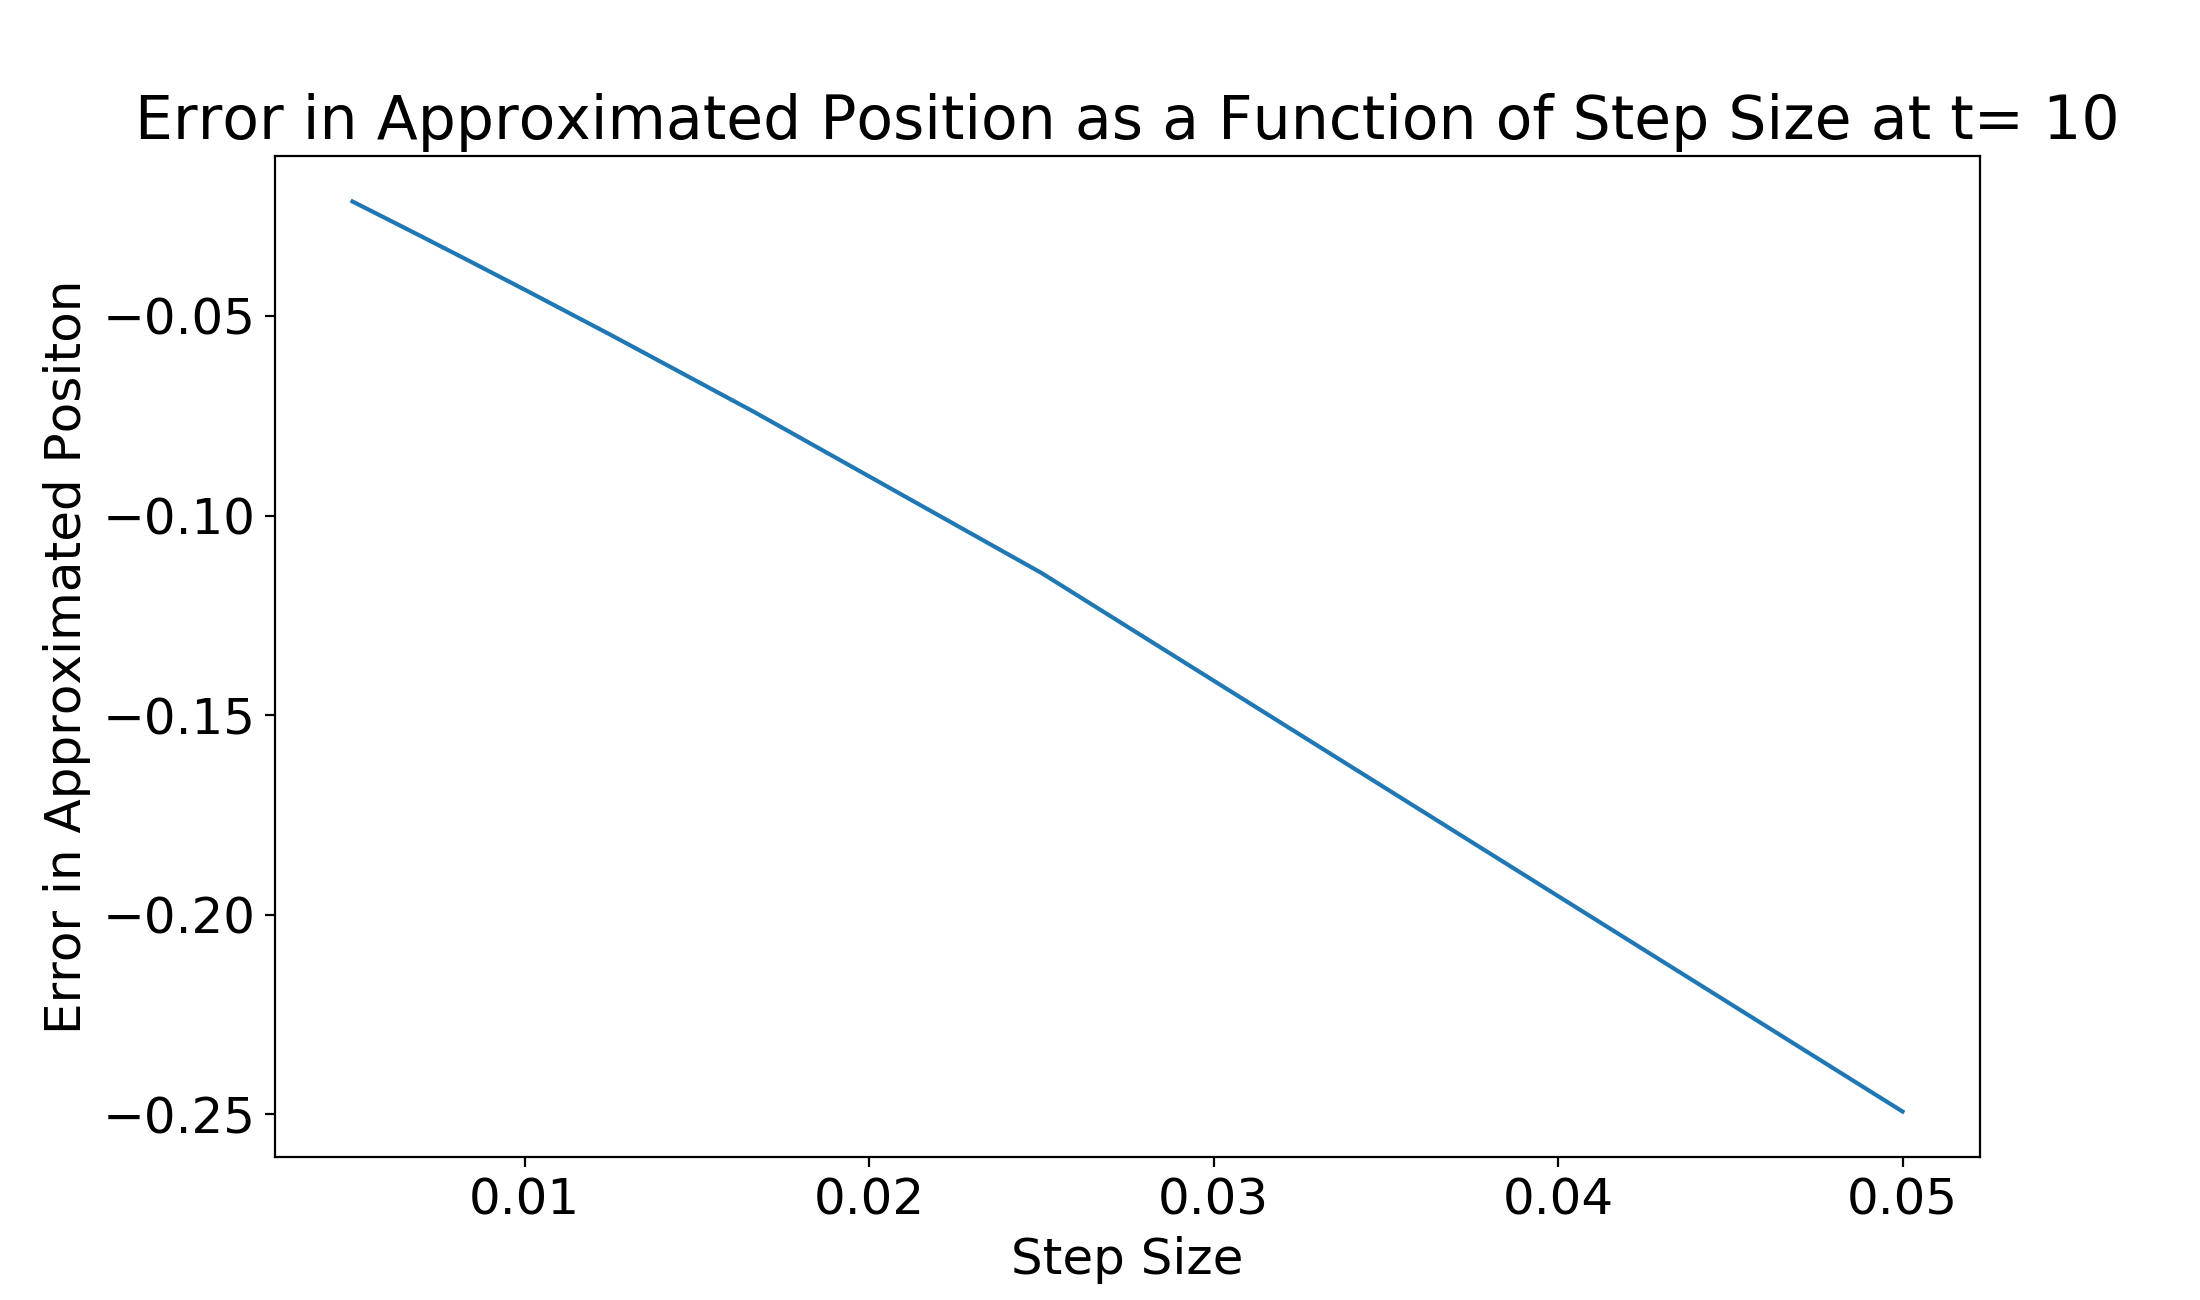
\includegraphics[width=.75\linewidth]{hVsErrExp.png}
\caption{}
\end{figure}

Note that although error is decreasing as step size increases, the magnitude of error is still increasing. This result is thus consistent with the intuition that performing more calculations should allow for more accurate approximations. Also note that the graph is roughly linear, which is consistent with the error being directly proportional to the step size.
\end{problem}

\begin{problem}{4}
As was noted in problem 1, the approximations given by the explicit Euler's function implies that the system is increasing in energy, which is not correct. In figure 3, we see how this increasing energy is coupled with increasing errors in position and velocity for a spring with $x_i=1$ and $v_i=0$.

\begin{figure}[h]
\centering
\begin{subfigure}{.3\textwidth}
  \centering
  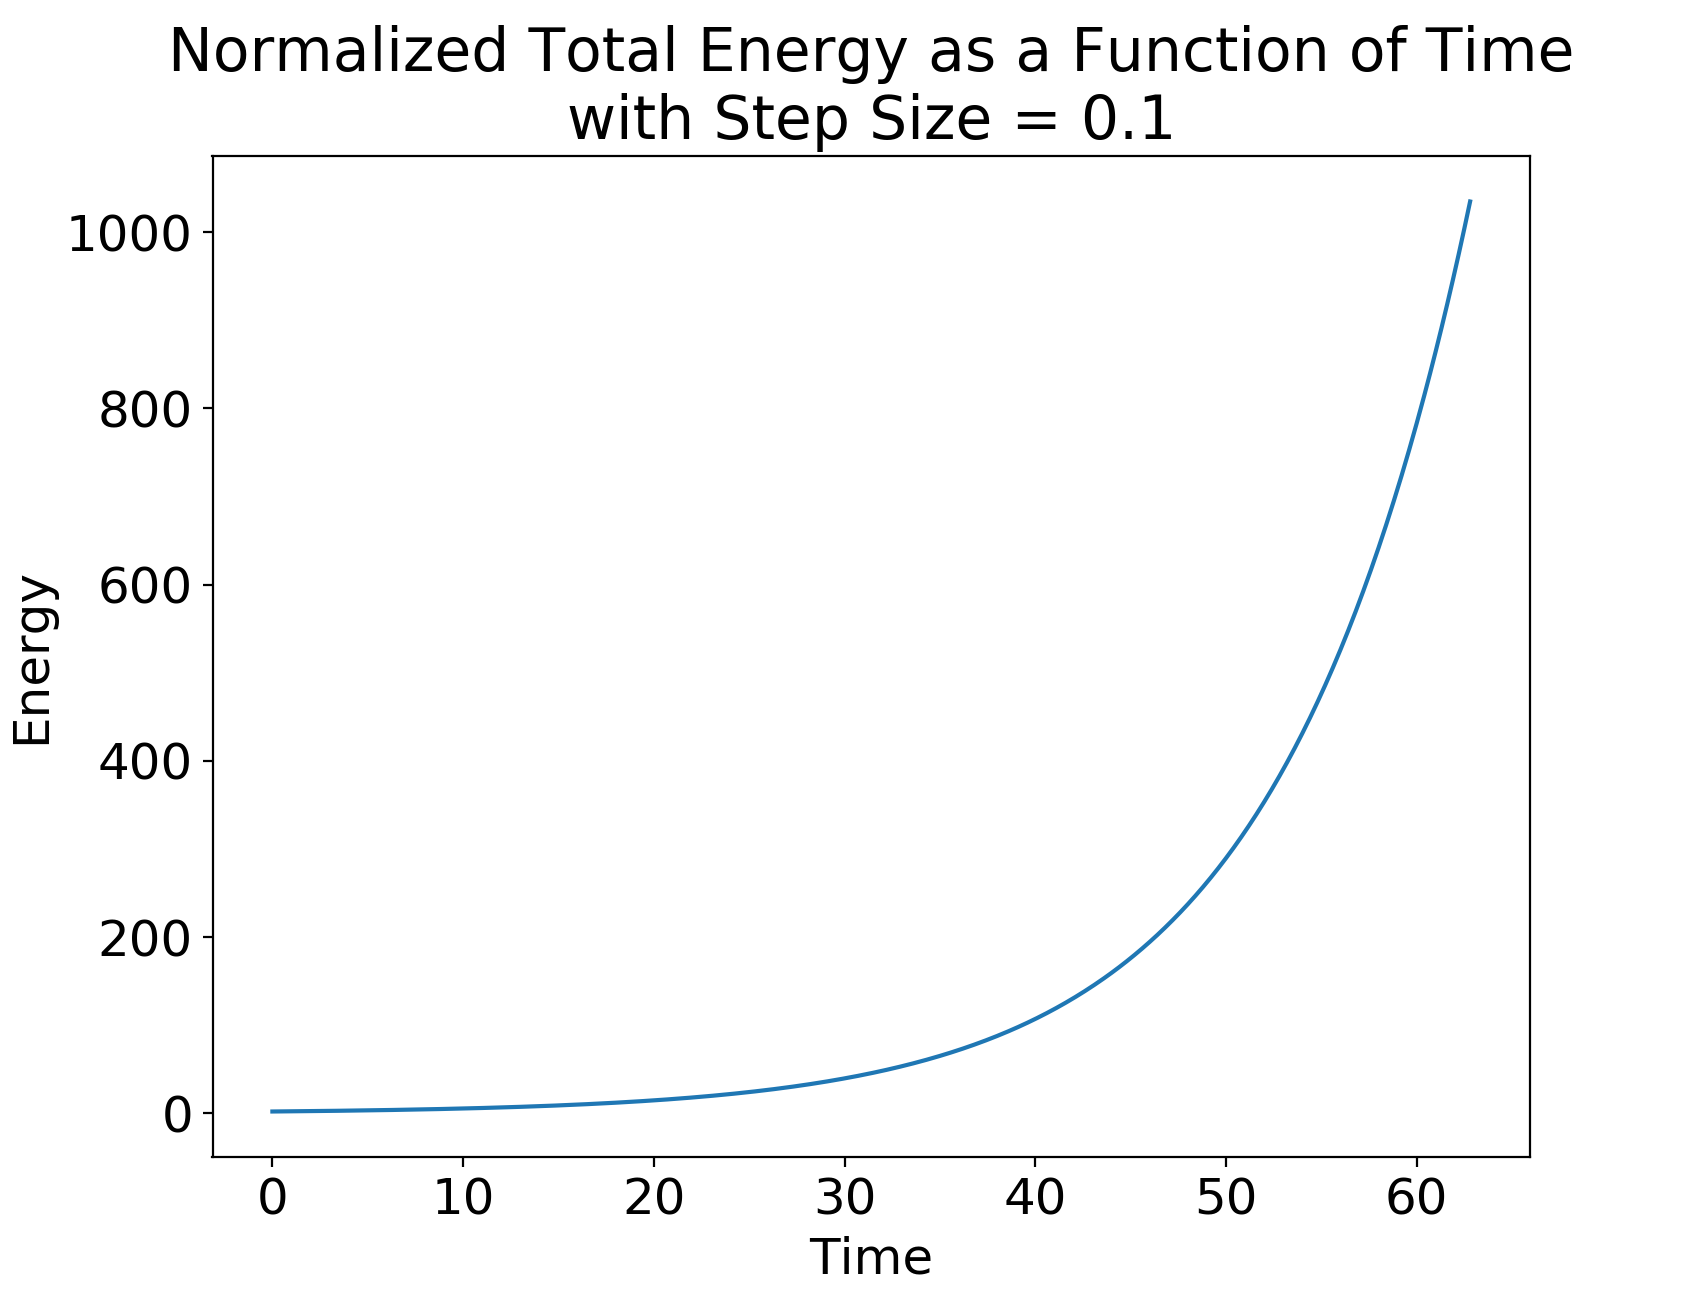
\includegraphics[width=1\linewidth]{NrgExp.png}
\end{subfigure}%
\begin{subfigure}{.3\textwidth}
  \centering
  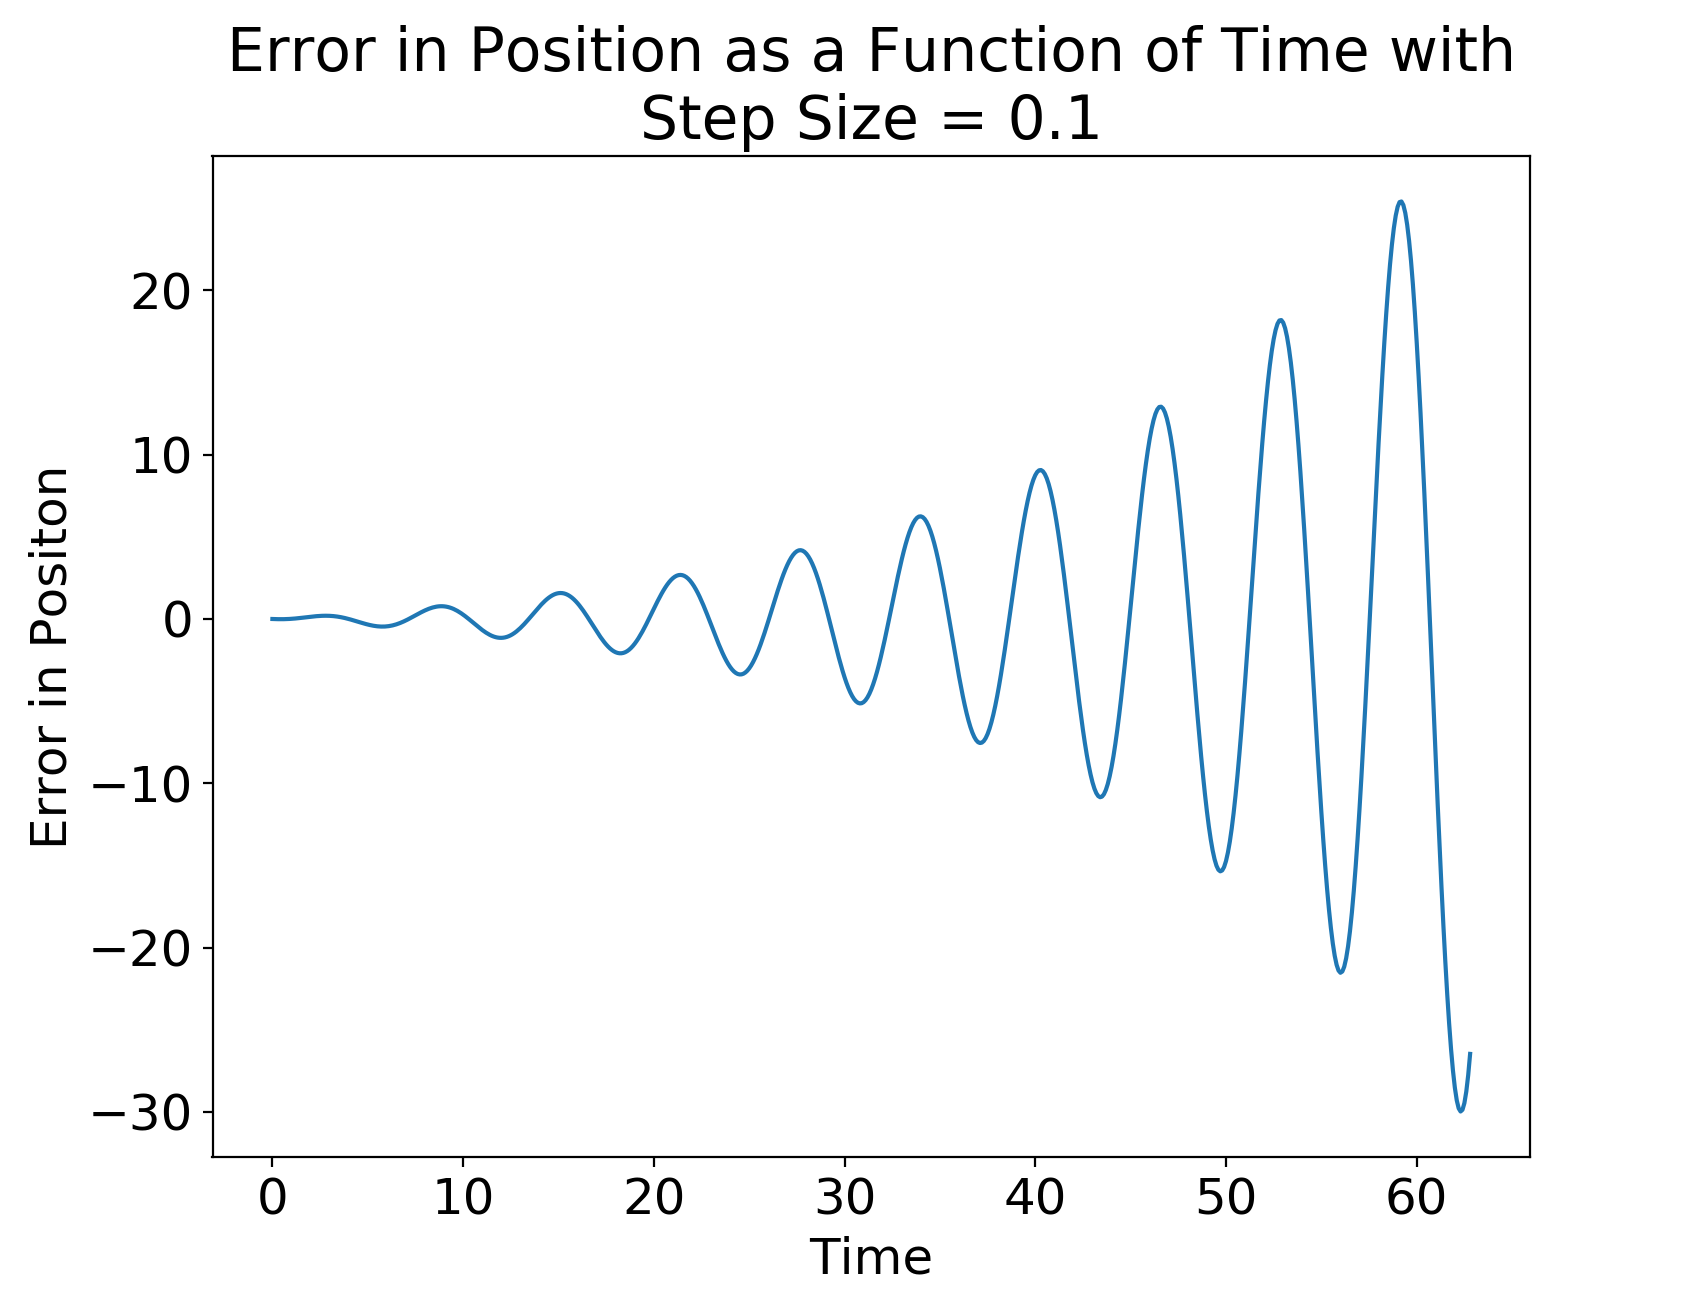
\includegraphics[width=1\linewidth]{ErrPosExp.png}
\end{subfigure}
\begin{subfigure}{.3\textwidth}
  \centering
  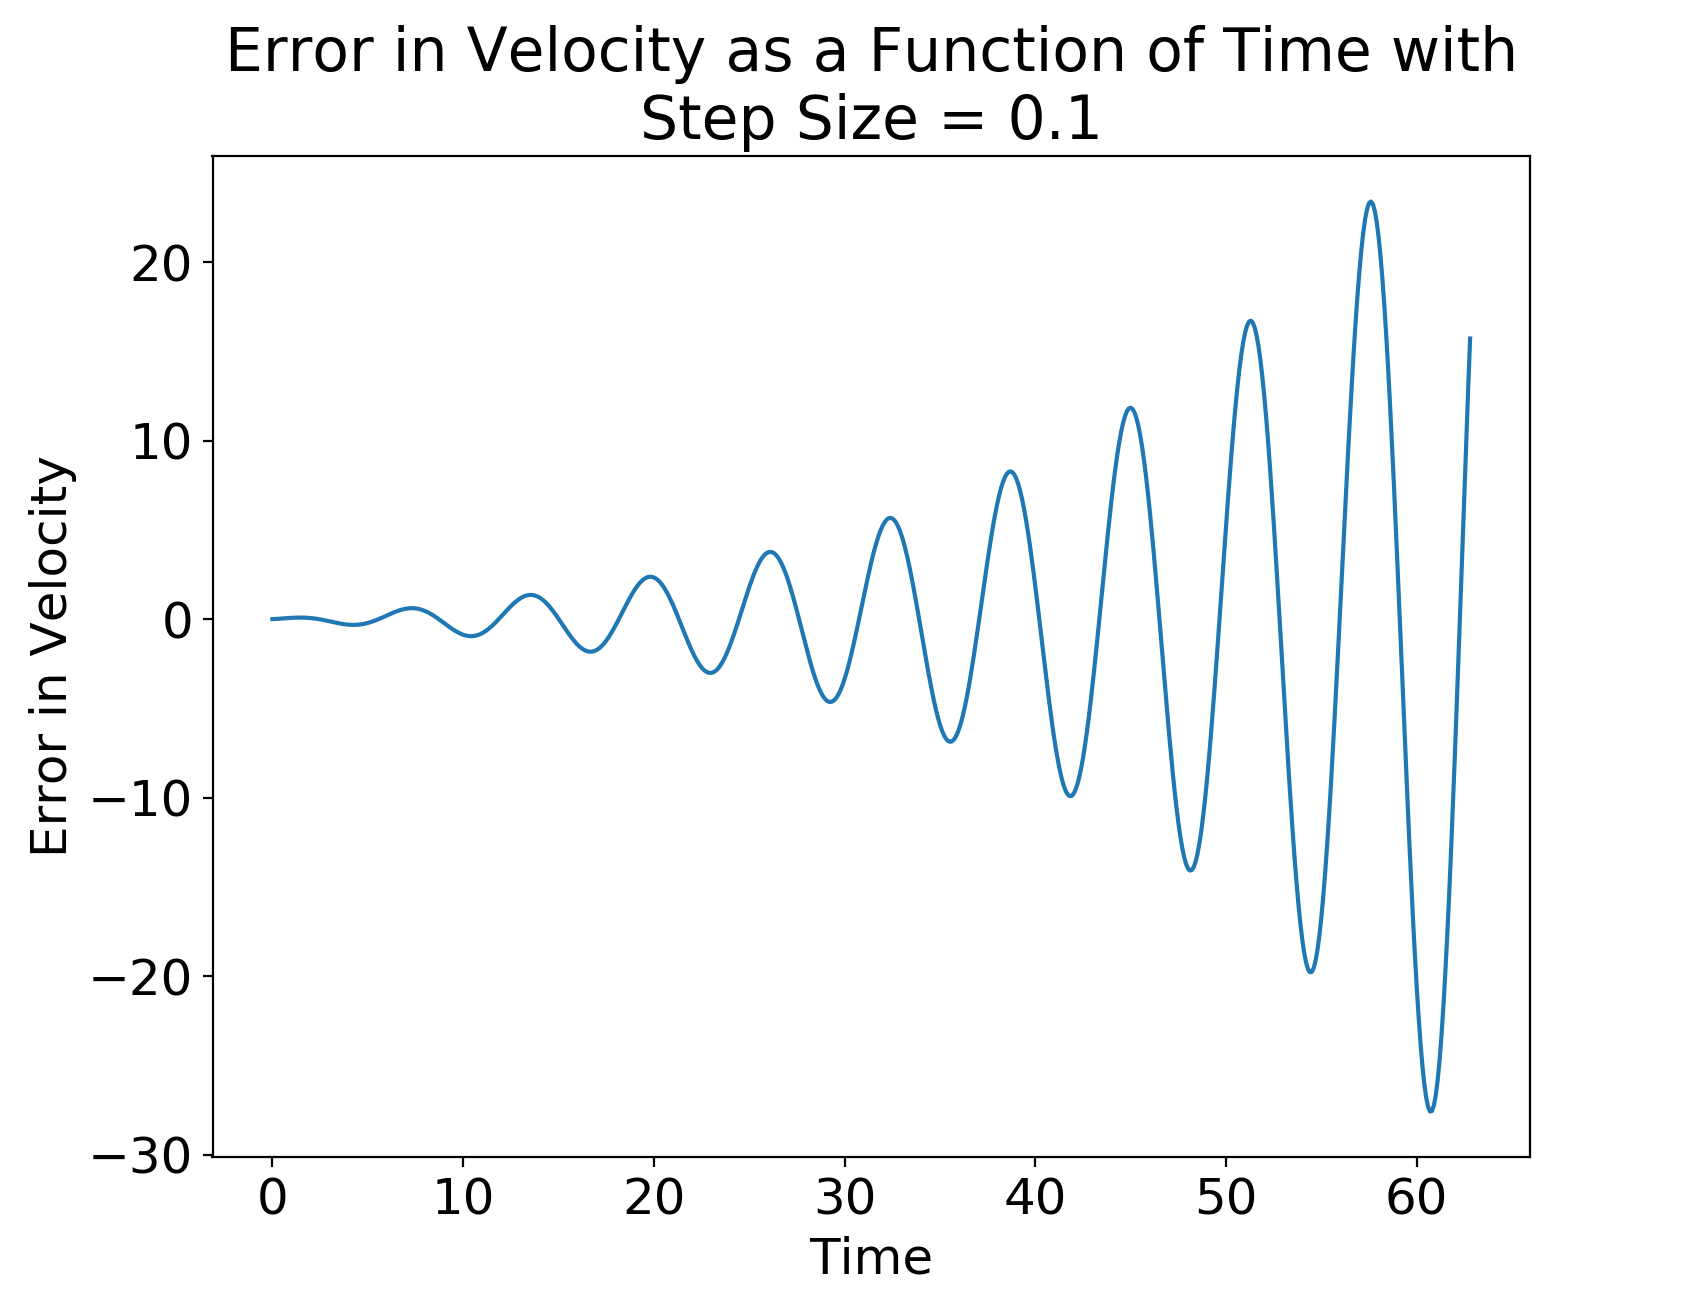
\includegraphics[width=1\linewidth]{ErrVelExp.png}
\end{subfigure}
\caption{Normalized Global Energy and Approximation Errors for Explicit Euler's Method}
\end{figure}

As expected, the errors in both position and velocity increase over time. Also, given that position and velocity remain in a stable range over time, it makes sense that the error in the approximations appears to grow at a similar rate to the approximations themselves (as seen in figure 1). Also, given that energy scales with position and velocity squared, it makes sense that the energy appears to increase with a more pronounced concavity than the increases in position and velocity.
\end{problem}

\begin{problem} {5}
Using the implicit Euler's method, which gives that $x_{i+1}=x_i+hv_{i+1}$ and $v_{i+1}=v_i-hx_{i+1}$, it can be found that $x_{i+1}=\frac{x_i+hv_i}{1+h^2)}$ and $v_{i+1}=\frac{x_i-hx_i}{1+h^2)}$. With the implicit Euler's method, the position and velocity of a spring (with $\frac{k}{m}=$, $x_i=-1$, and $v_i=1$) as a function of time were approximated, as shown in figure 4.

\begin{figure}[h]
\centering
\begin{subfigure}{.45\textwidth}
  \centering
  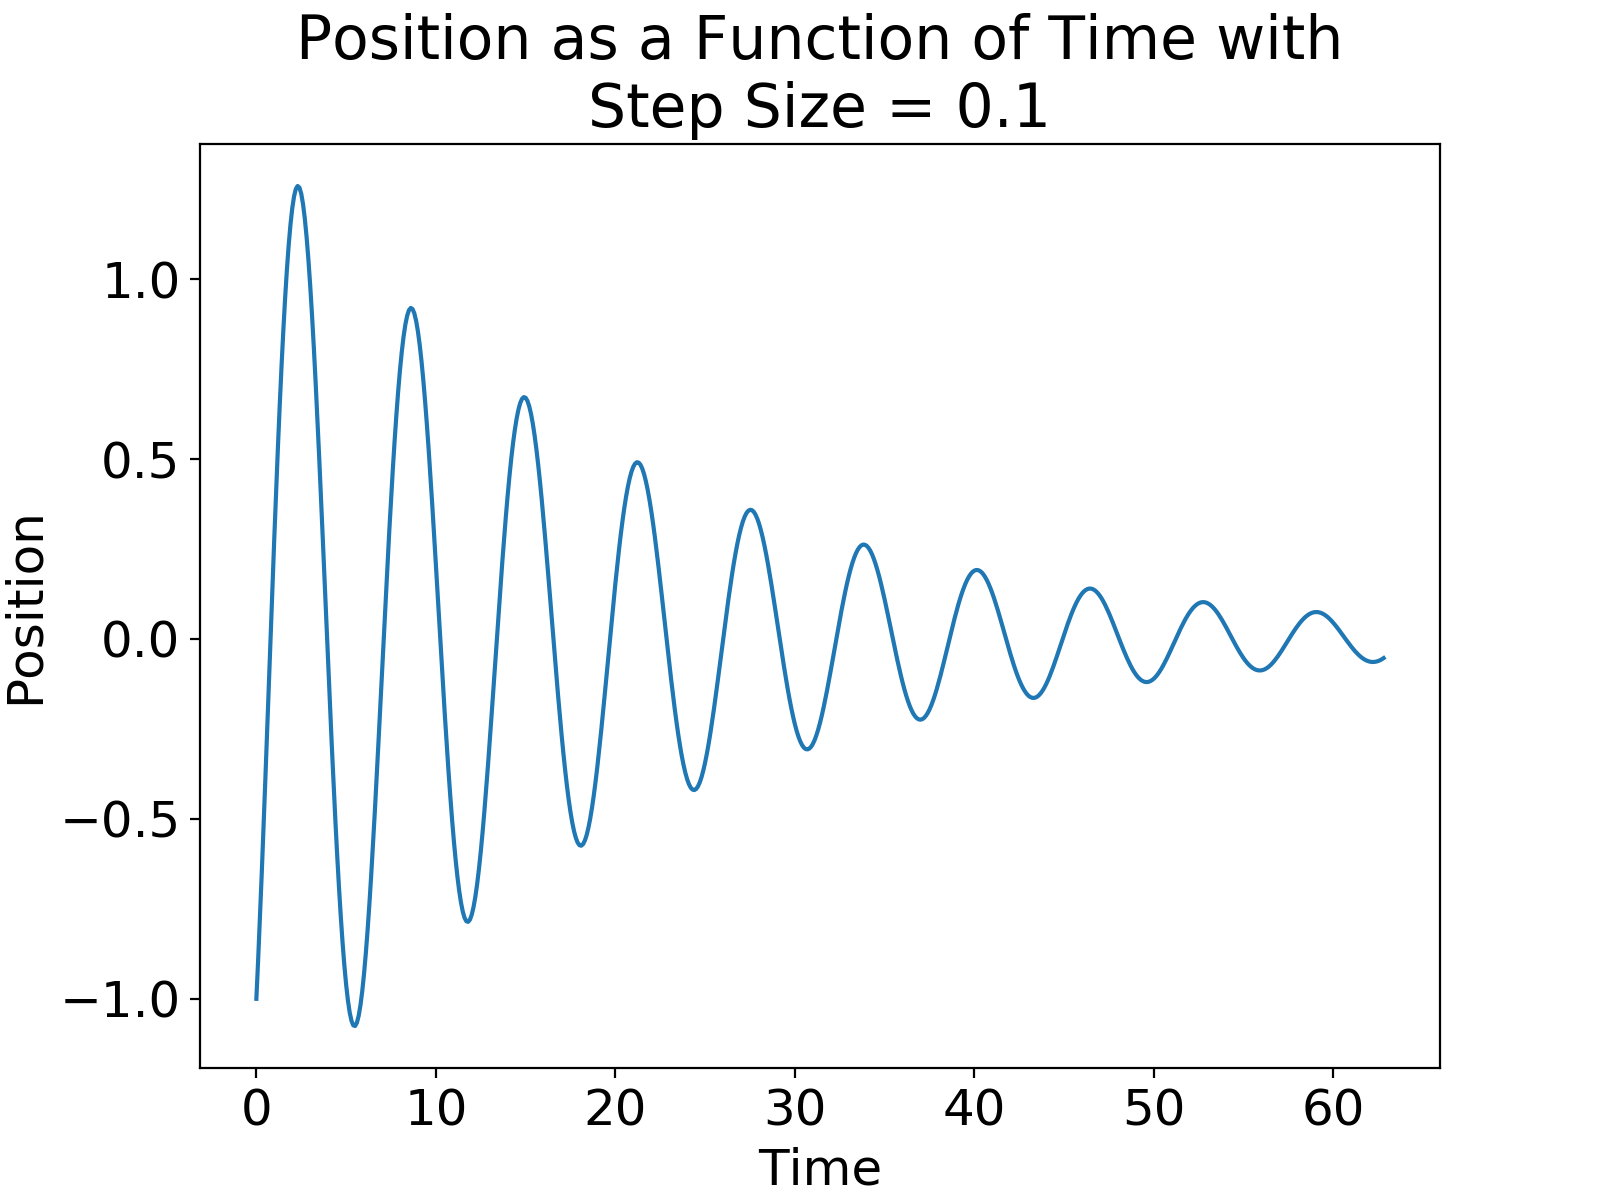
\includegraphics[width=1\linewidth]{PosImp.png}
\end{subfigure}%
\begin{subfigure}{.45\textwidth}
  \centering
  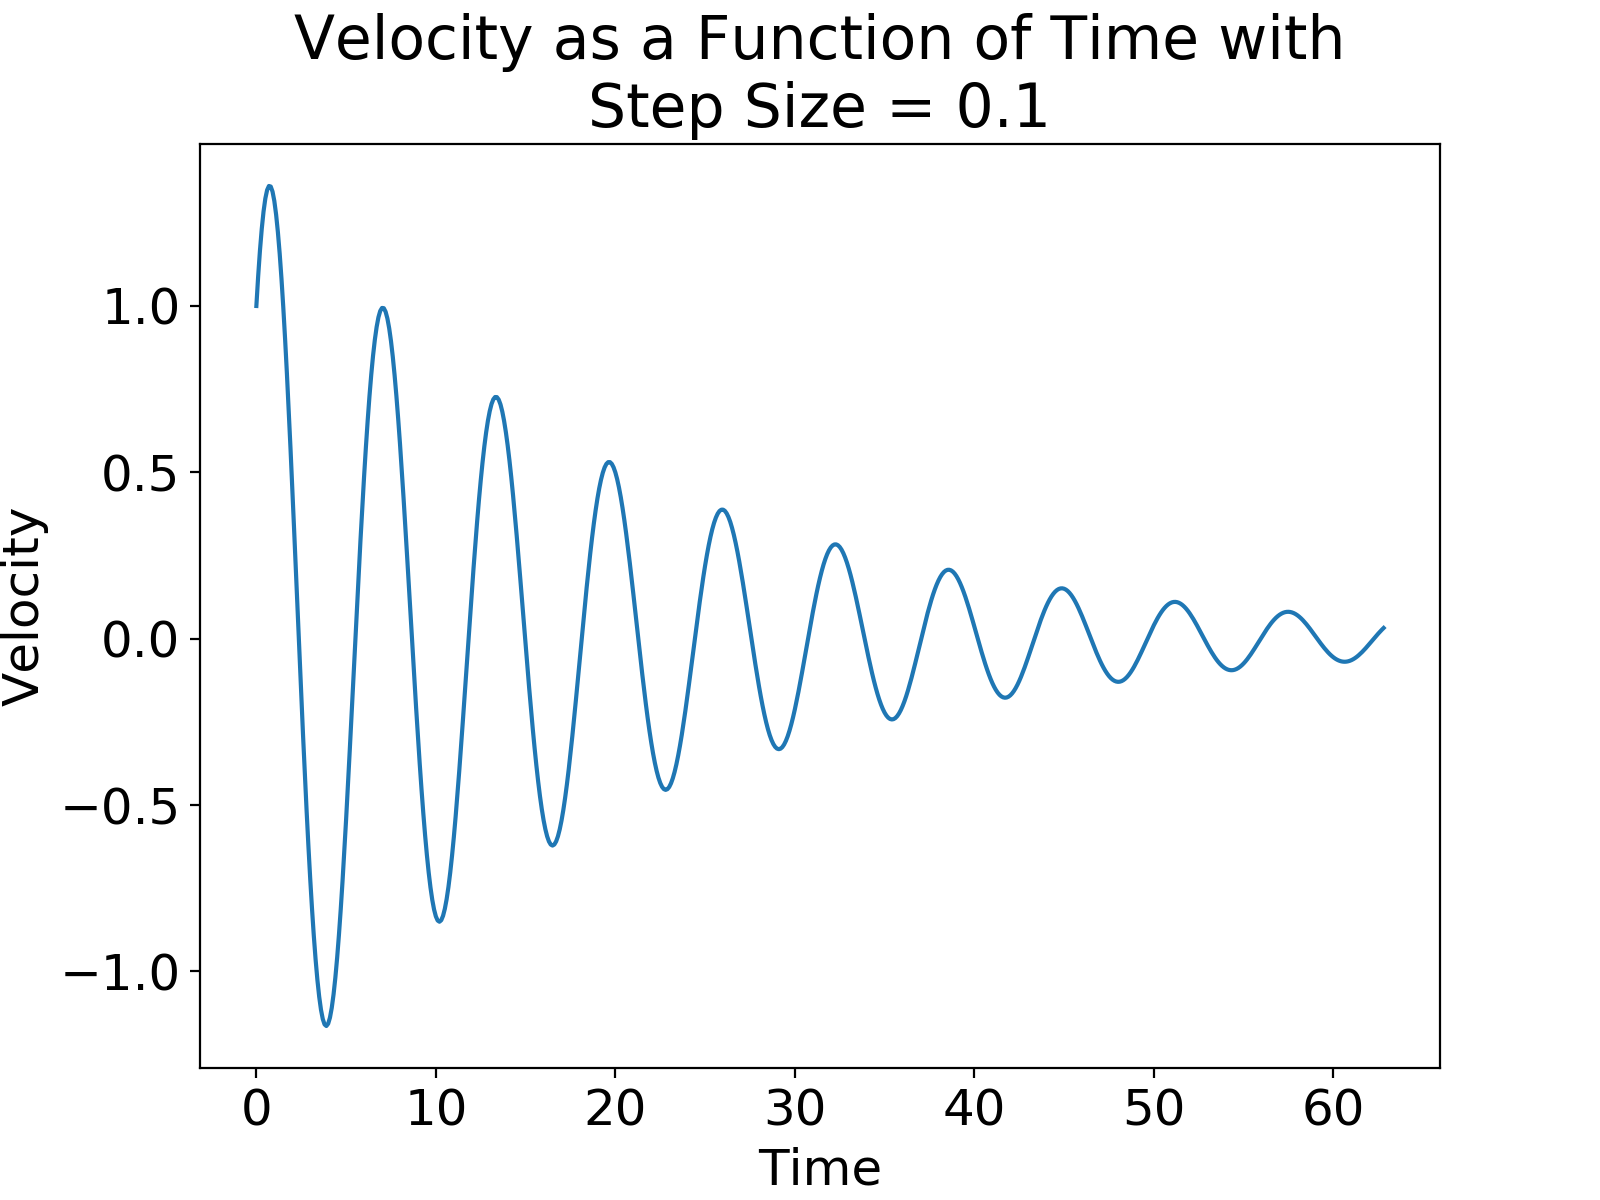
\includegraphics[width=1\linewidth]{VelImp.png}
\end{subfigure}
\caption{Position and Velocity as a Function of Time as Approximated Using the Implicit Euler's Method}
\end{figure}

Note that unlike in figure 1, with the implicit Euler's method, position and velocity appear to decrease with time, which would imply that the system is losing energy. This loss of energy can be observed in figure 5, alongside the errors in the approximations as a function of time.

\begin{figure}[h]
\centering
\begin{subfigure}{.3\textwidth}
  \centering
  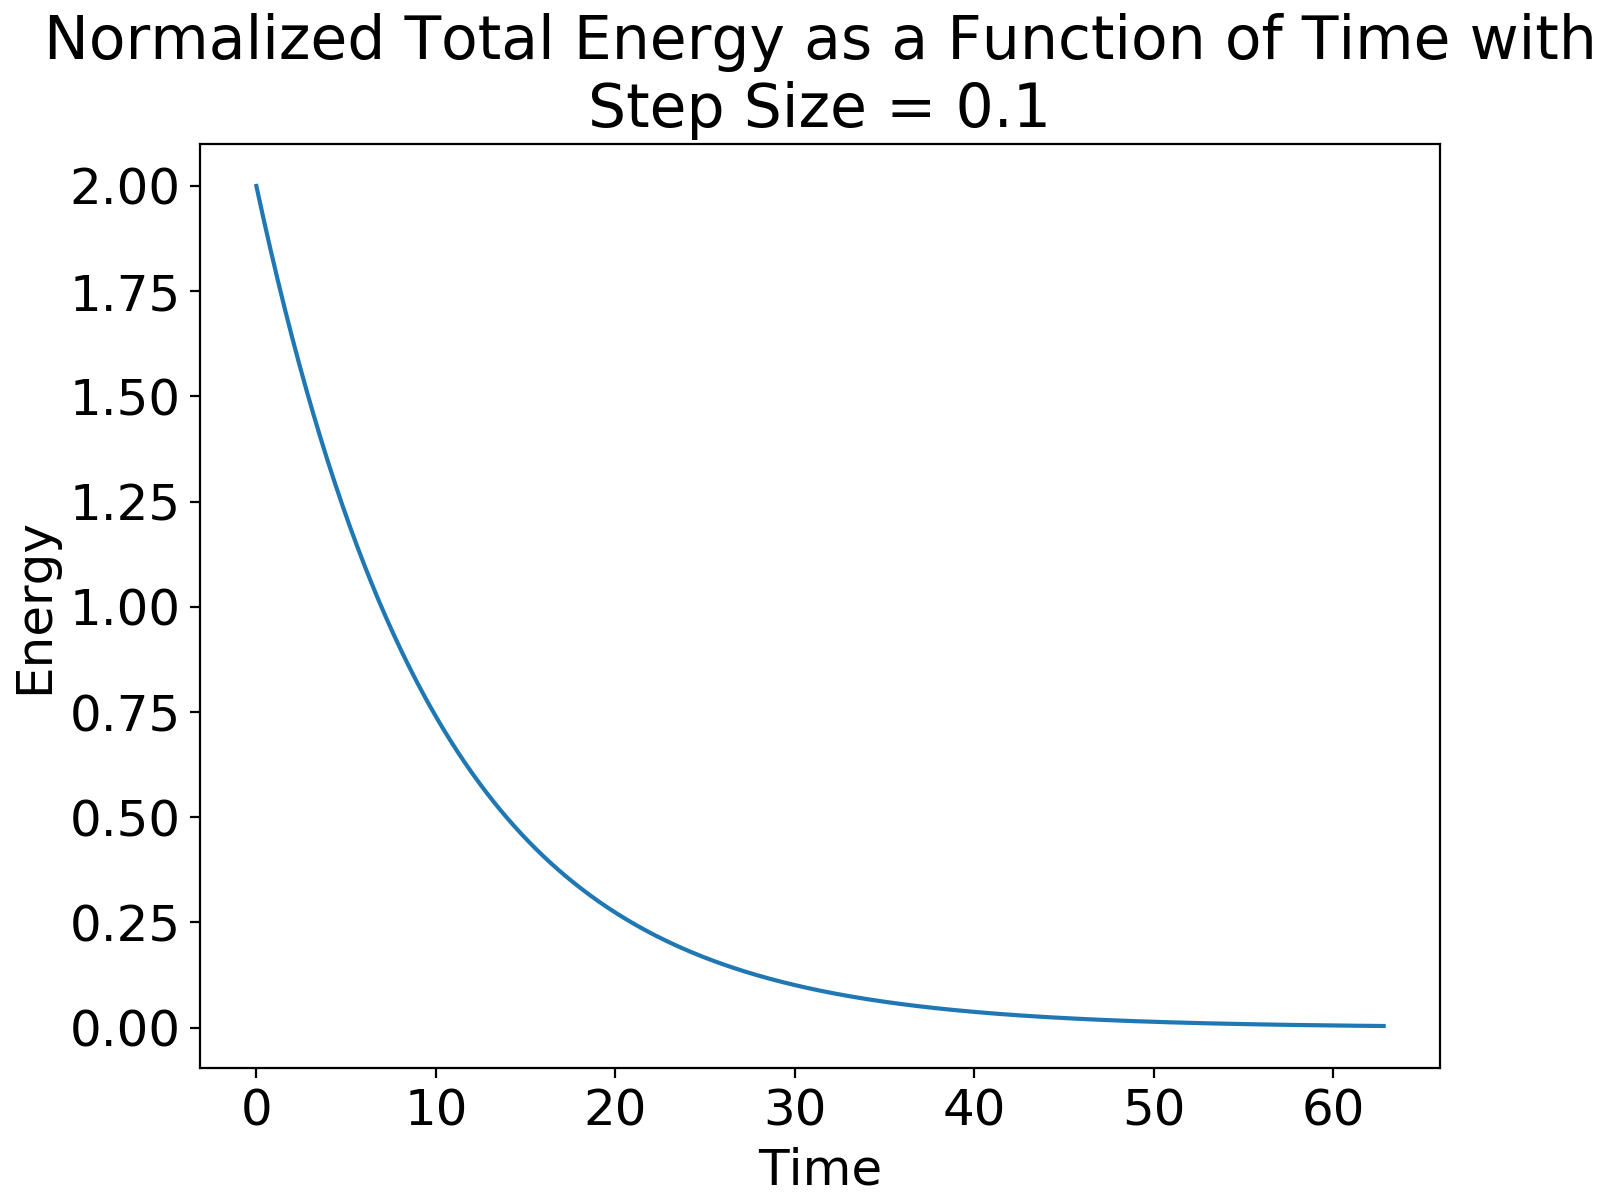
\includegraphics[width=1\linewidth]{NrgImp.png}
\end{subfigure}%
\begin{subfigure}{.3\textwidth}
  \centering
  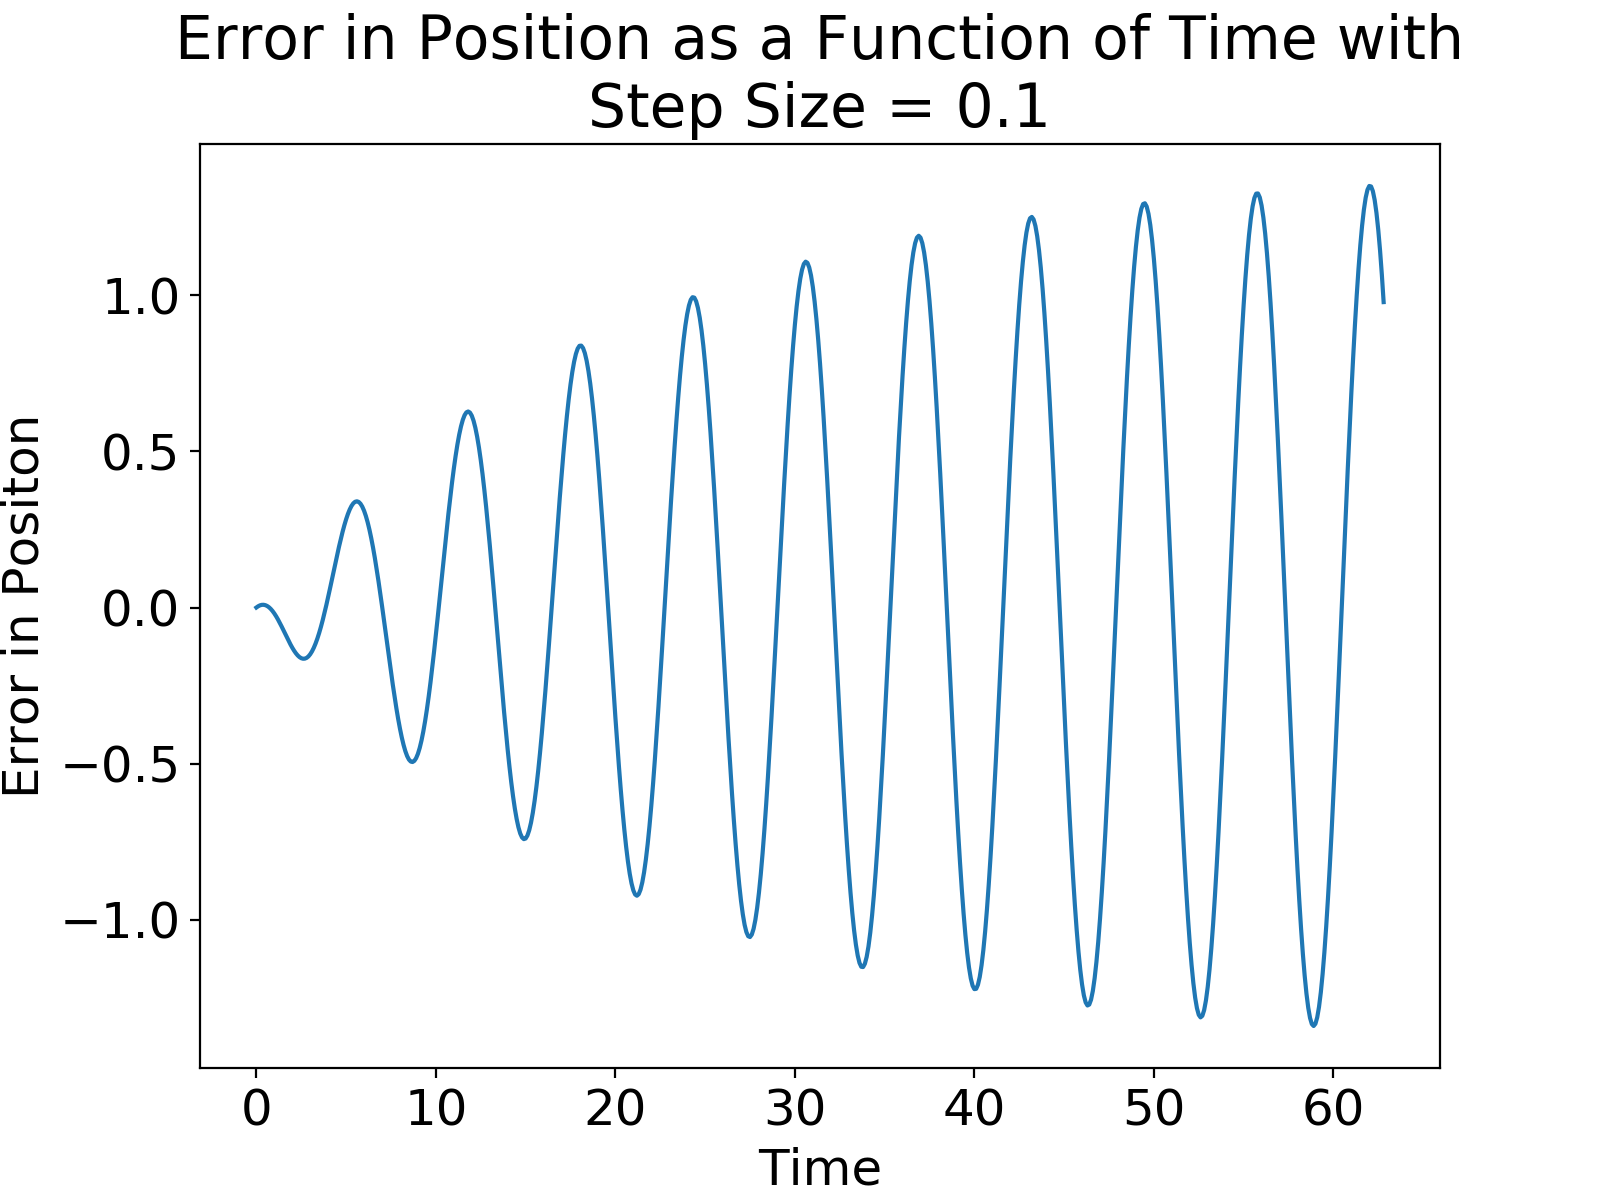
\includegraphics[width=1\linewidth]{ErrPosImp.png}
\end{subfigure}
\begin{subfigure}{.3\textwidth}
  \centering
  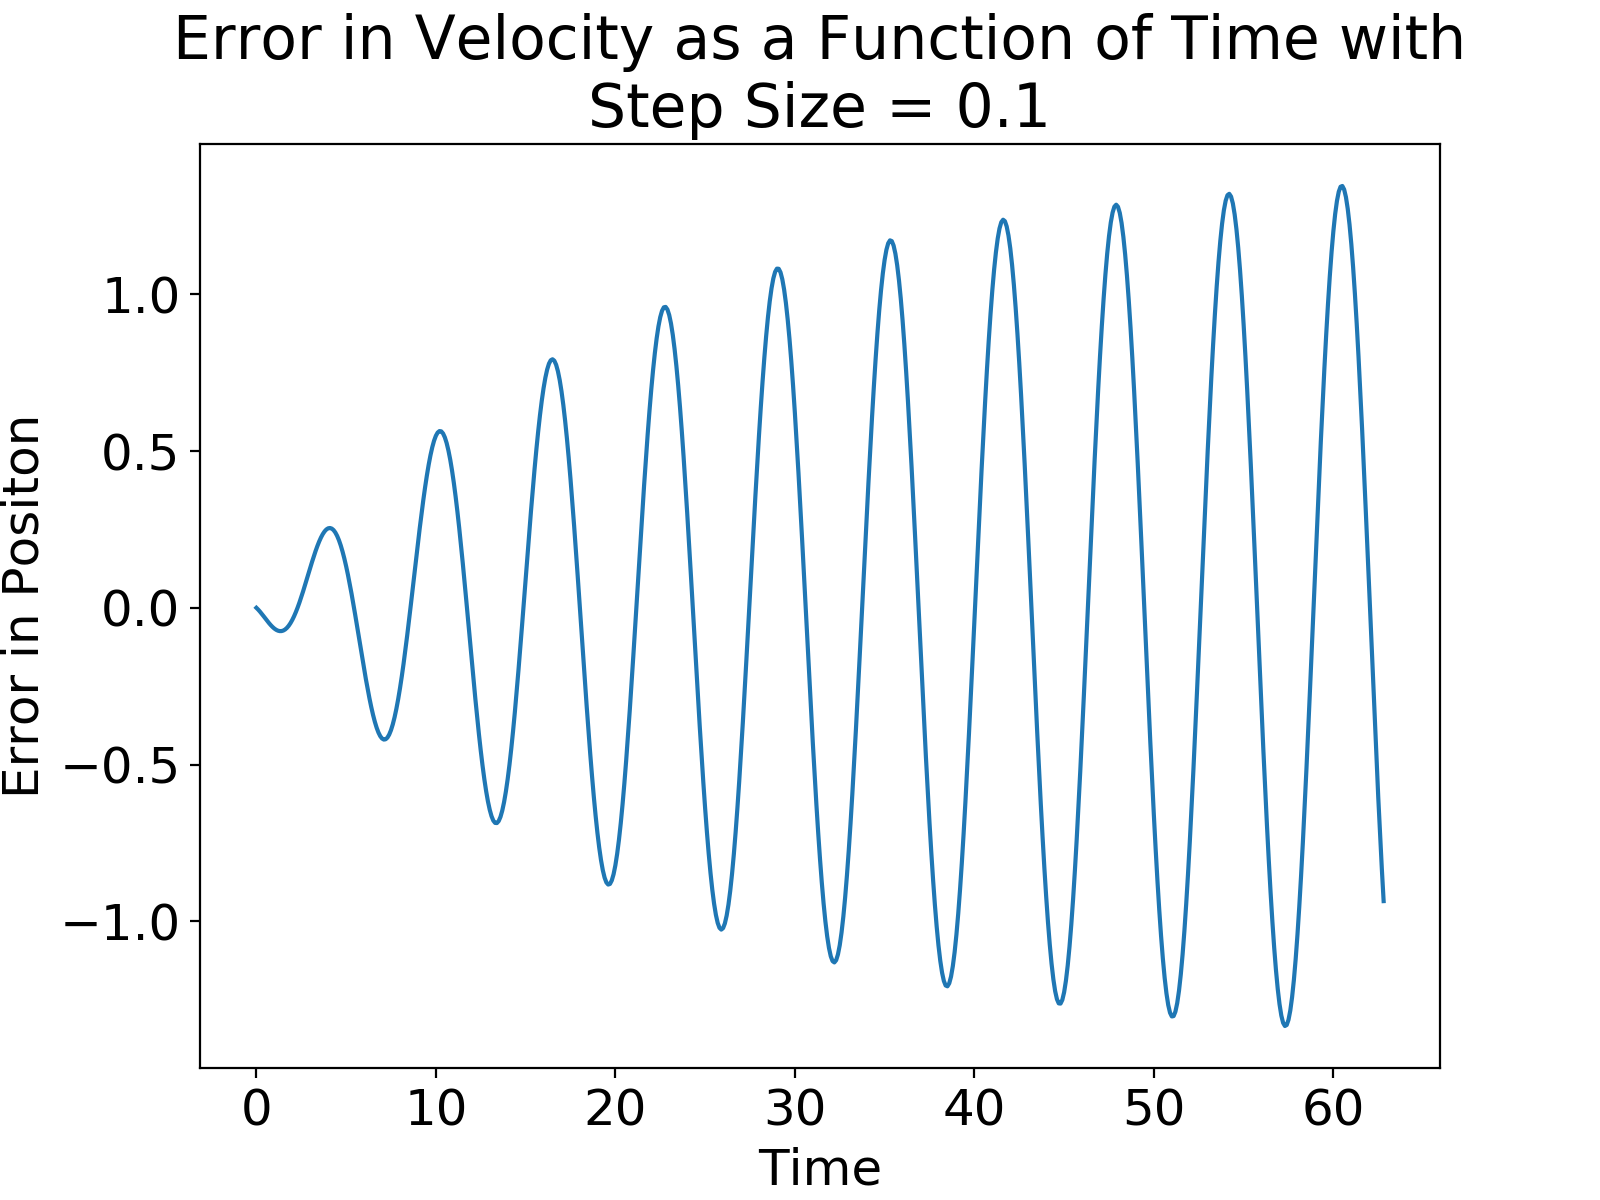
\includegraphics[width=1\linewidth]{ErrVelImp.png}
\end{subfigure}
\caption{Normalized Global Energy and Approximation Errors for Implicit Euler's Method}
\end{figure}

As expected, energy appears to decrease to zero as time increases. Also, observe that the peaks of error in position and velocity appear to be asymptotically approaching constant levels. This form is consistent with the fact that as the approximated values of position and velocity both go to zero, the error in those values cannot possibly be much more than the actual values, which are themselves stable at $\sqrt{v_i+x_i}=\sqrt{2}$ (as discussed in problem 3).
\end{problem}
\newpage

\begin{problem} {6}
Note that if we plot position versus velocity, the distance from a point to the origin will be of the form $\sqrt{x^2+v^2}=\sqrt{\text{Energy}}$. Thus, all points that have the same energy will all be the same distance from the origin (i.e. they will be arranged in a circle centered at the origin). The spring when modelled analytically is such a system with constant energy, and as can be seen in Figure 6, it's plot does in fact describe a circle centered at the origin. However, the systems as approximated using the explicit and implicit Euler's method do not have constant energy, and so are not circular. The explicit Euler's method gives a system with increasing energy, and so the points of the plot spiral outwards, while the implicit Euler's method gives one with decreasing energy, and so spirals inwards, both of which are also shown in Figure 6.
\begin{figure}[h]
\centering
\begin{subfigure}{.3\textwidth}
  \centering
  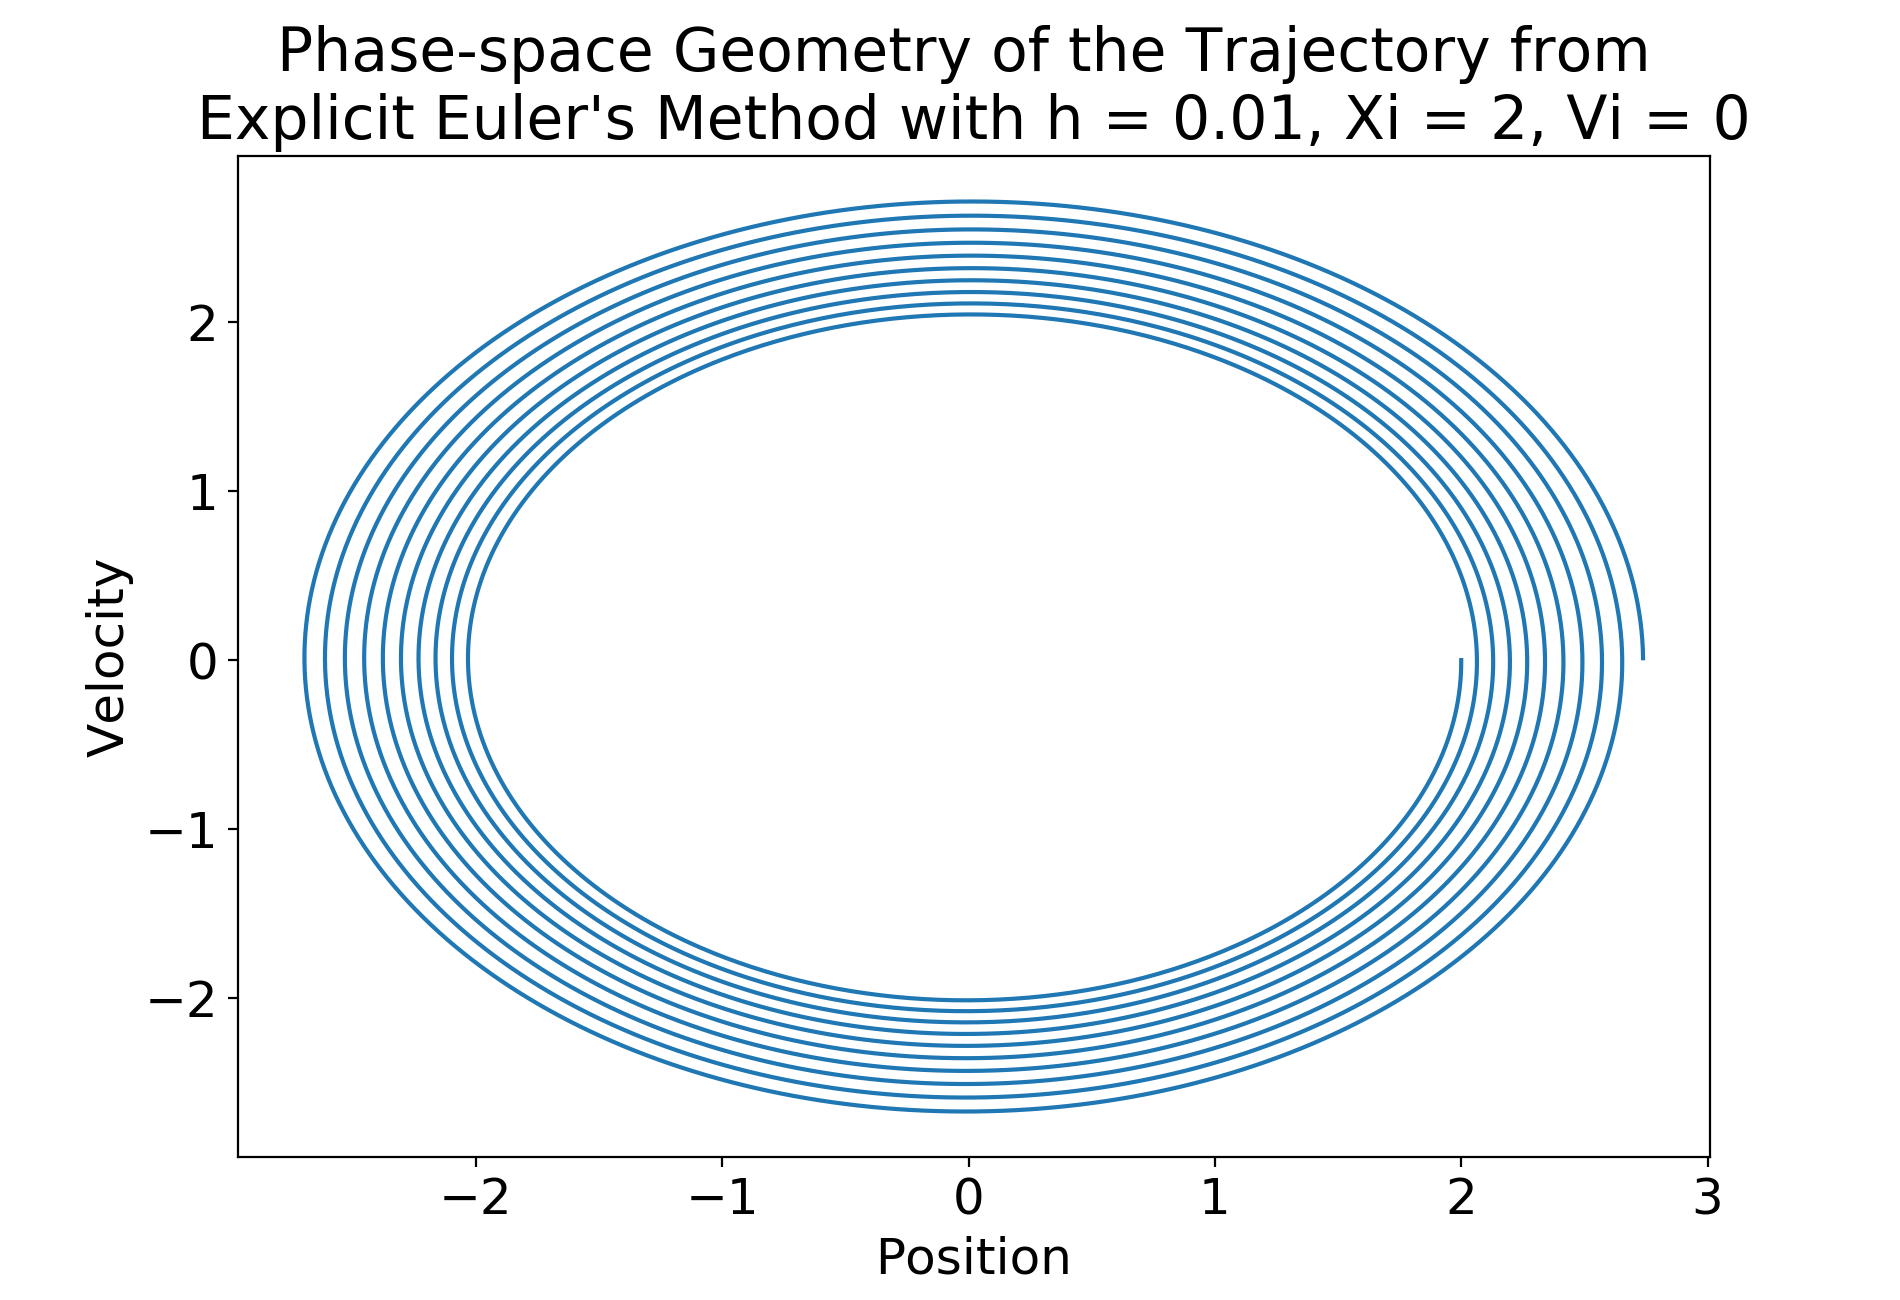
\includegraphics[width=1\linewidth]{PSGeoExp.png}
\end{subfigure}%
\begin{subfigure}{.3\textwidth}
  \centering
  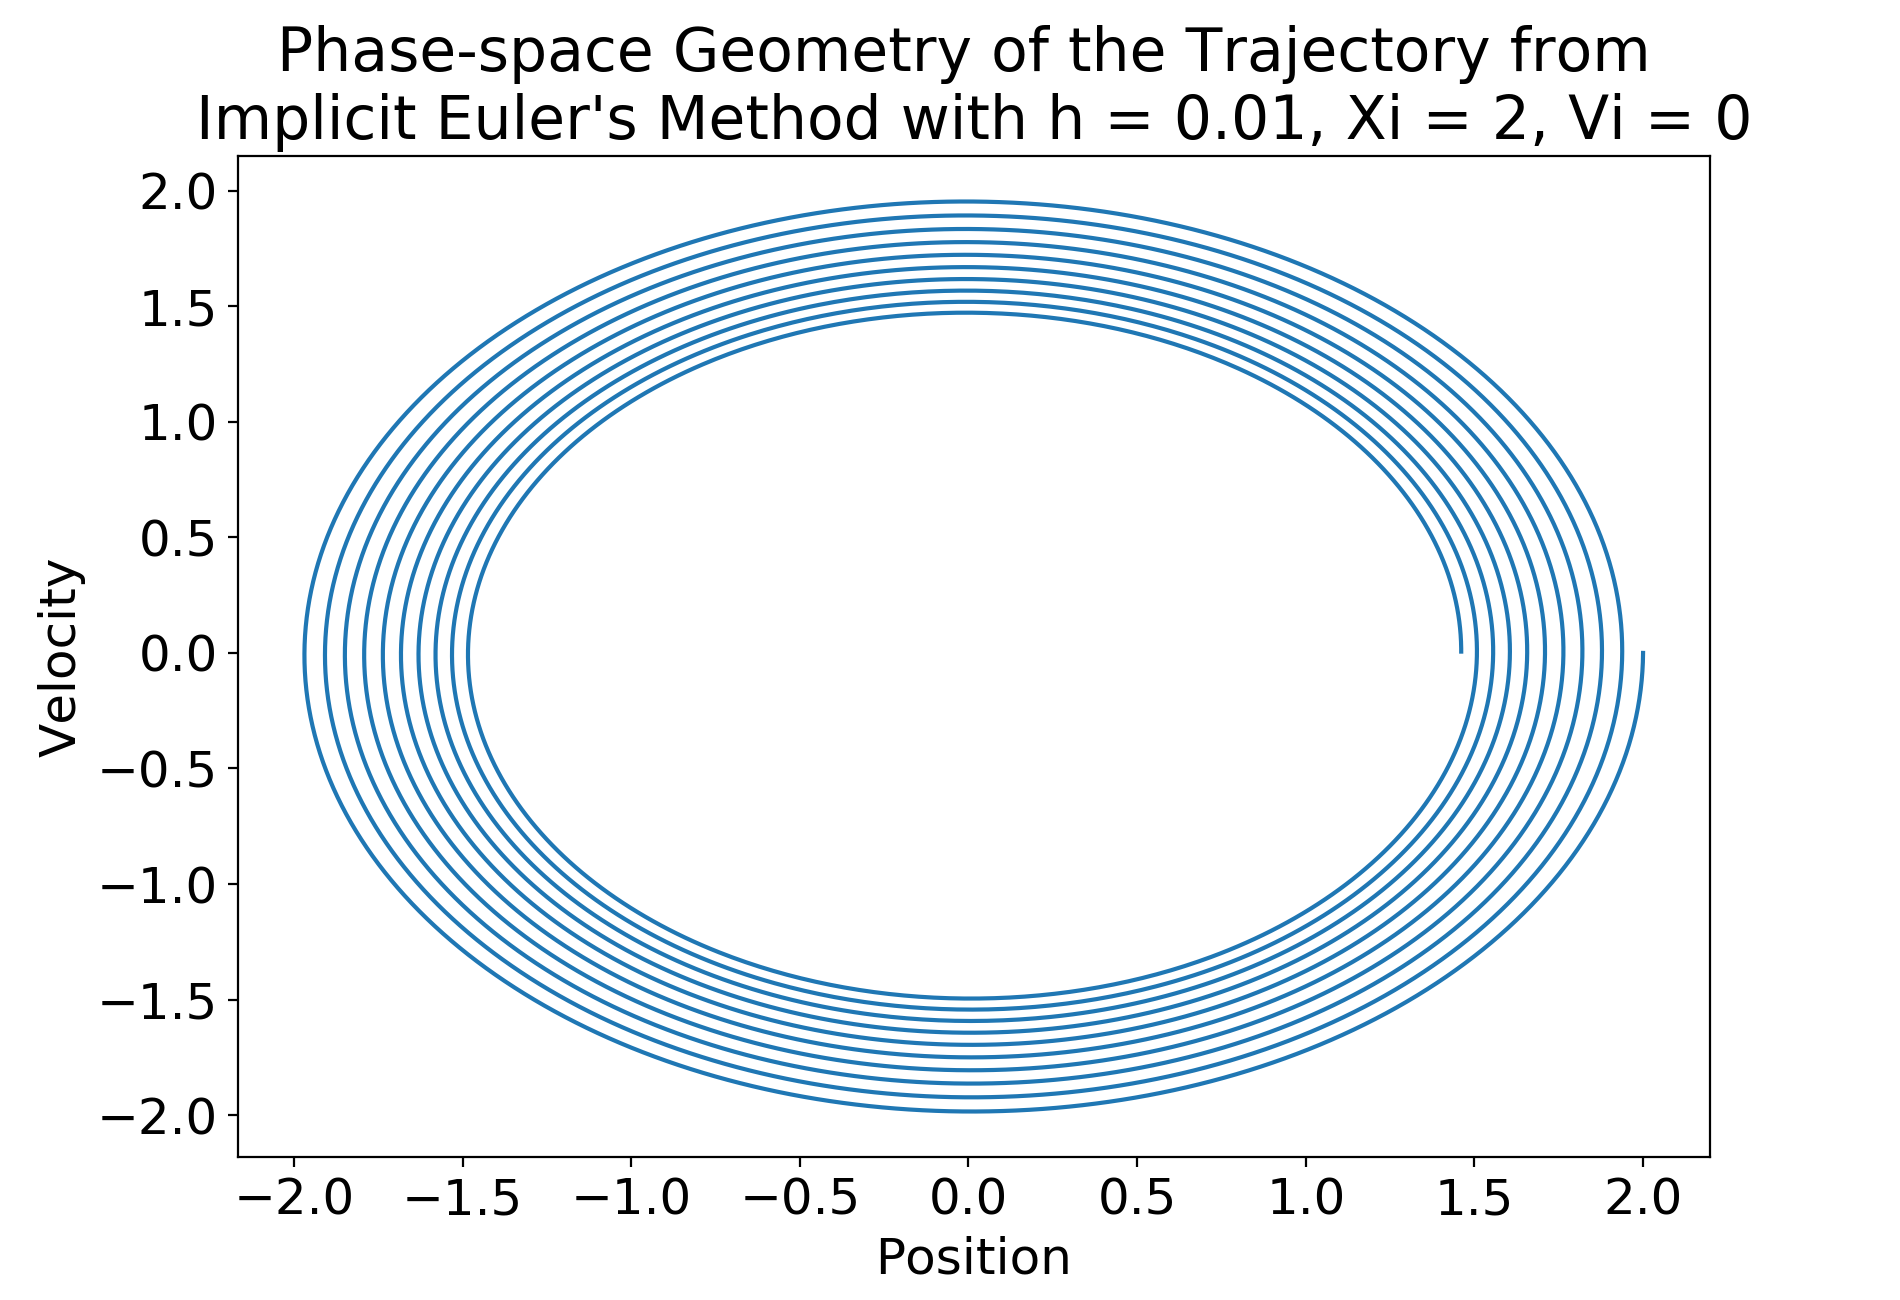
\includegraphics[width=1\linewidth]{PSGeoImp.png}
\end{subfigure}
\begin{subfigure}{.3\textwidth}
  \centering
  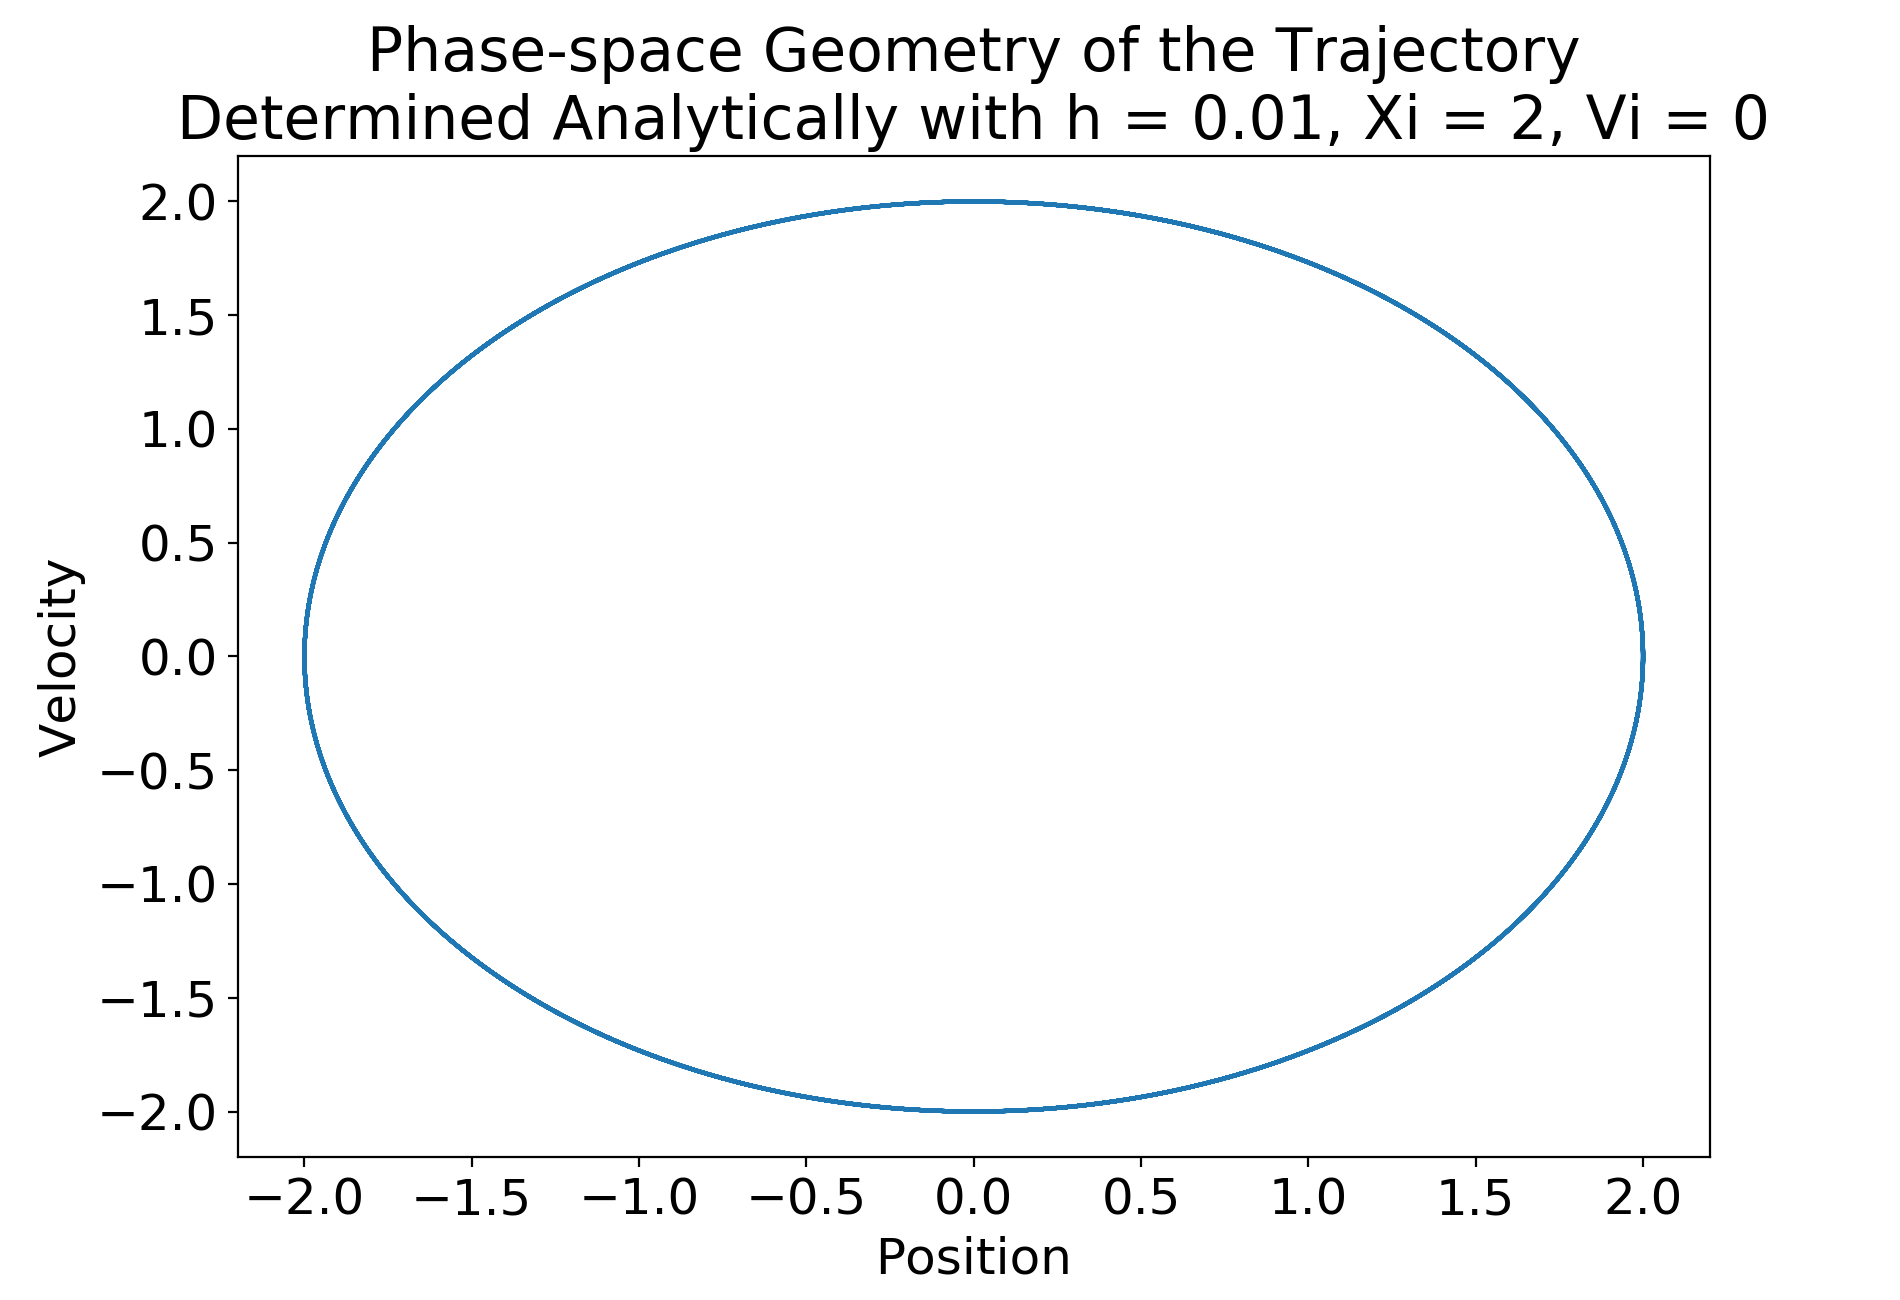
\includegraphics[width=1\linewidth]{PSGeoAna.png}
\end{subfigure}
\caption{Evolution of a Spring's Approximate and Analytic Position and Velocity}
\end{figure}
\end{problem}

\begin{problem} {7}
In contrast to the explicit and implicit Euler's methods, the symplectic Euler's method conserves energy well. At a step size of $0.01$, it appears indistinguishable from the analytic plot. Furthermore, even as that step size is increased dramatically, the approximated energy of the system does not tend to increase or decrease from cycle to cycle, and instead mostly corrects itself within a given cycle by producing somewhat more eccentric plots.

\begin{figure}[h]
\centering
\begin{subfigure}{.3\textwidth}
  \centering
  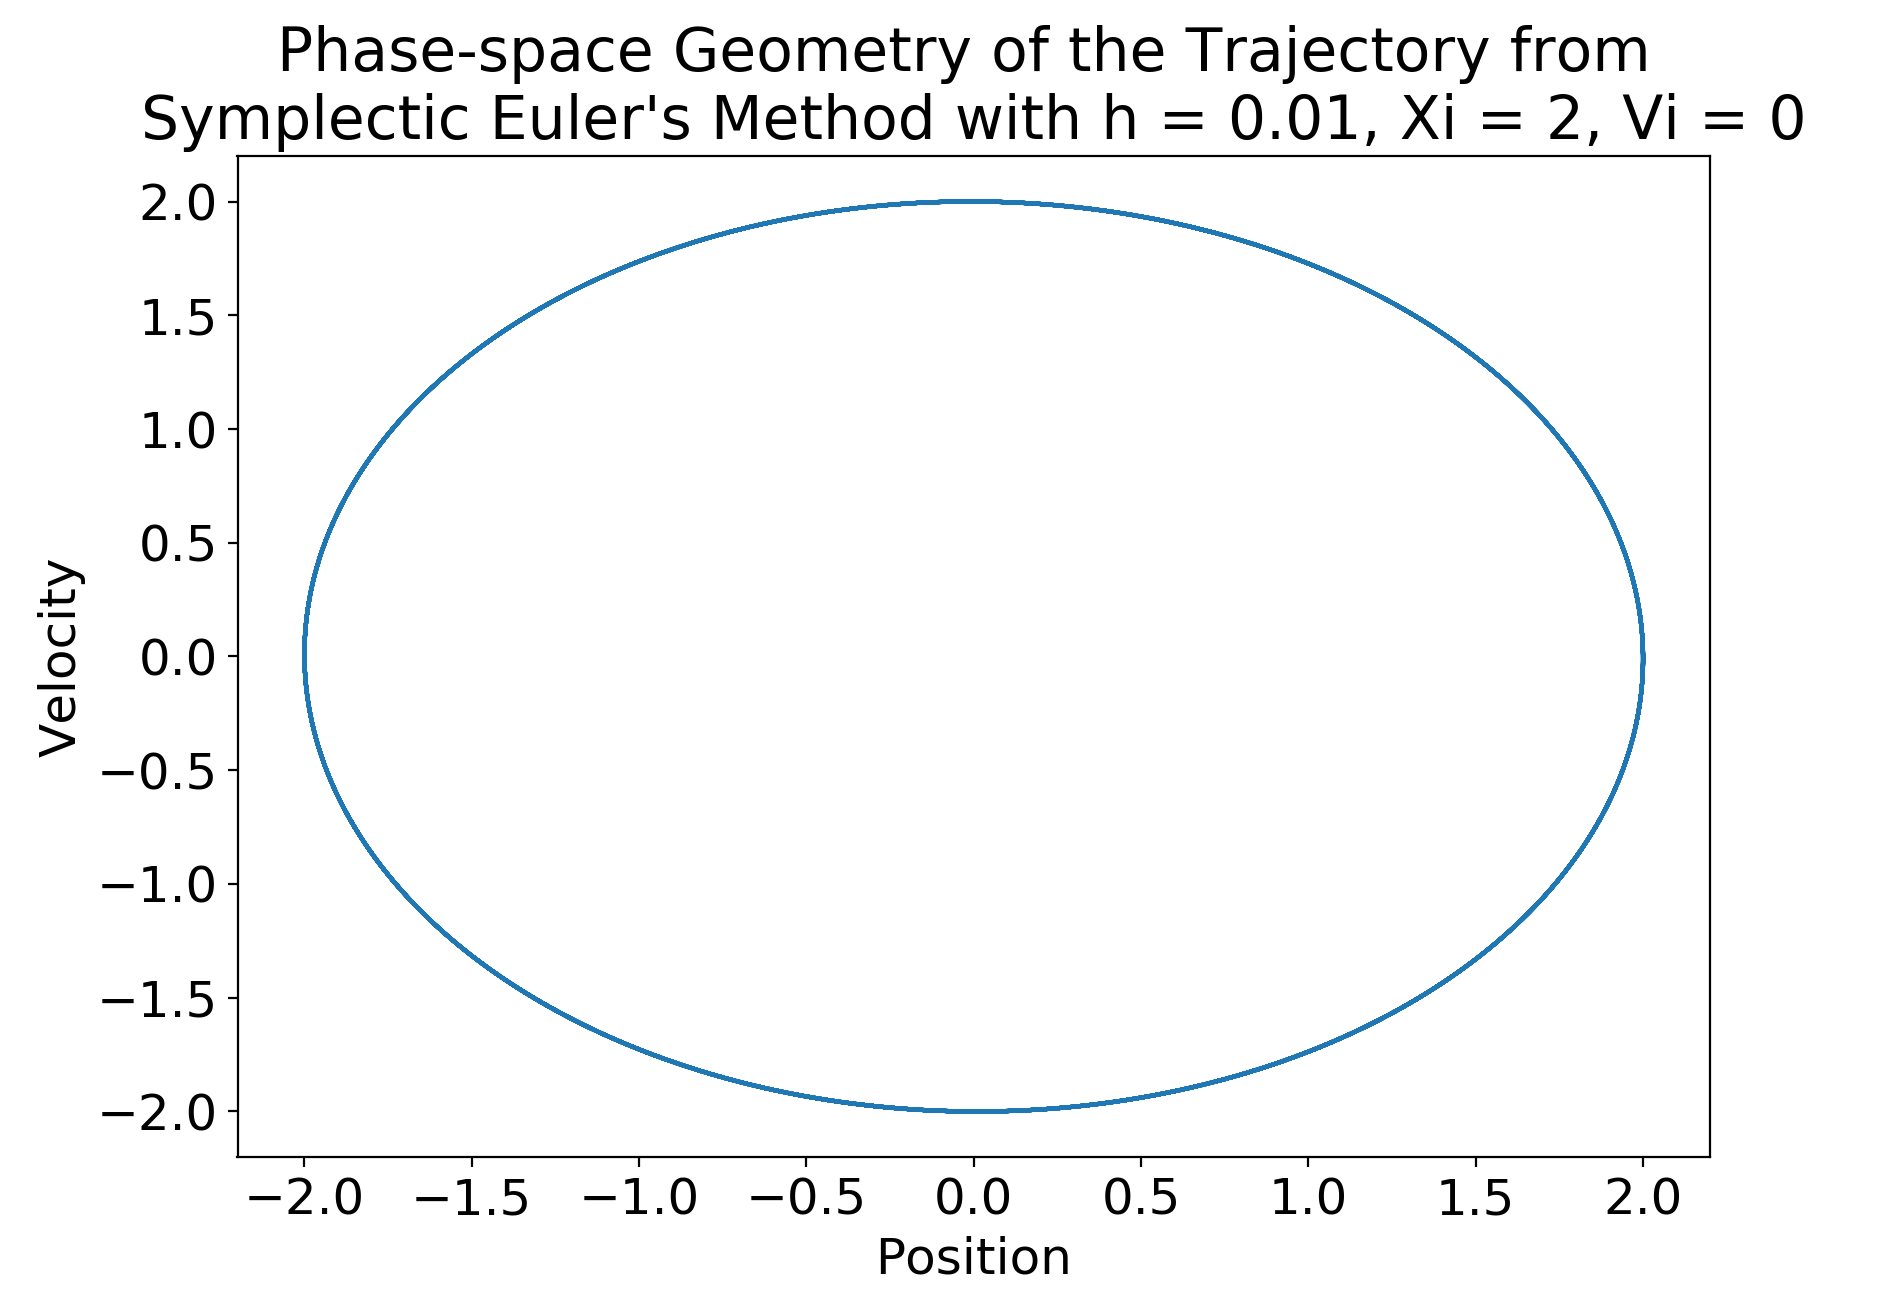
\includegraphics[width=1\linewidth]{PSGeoSym01.png}
\end{subfigure}%
\begin{subfigure}{.3\textwidth}
  \centering
  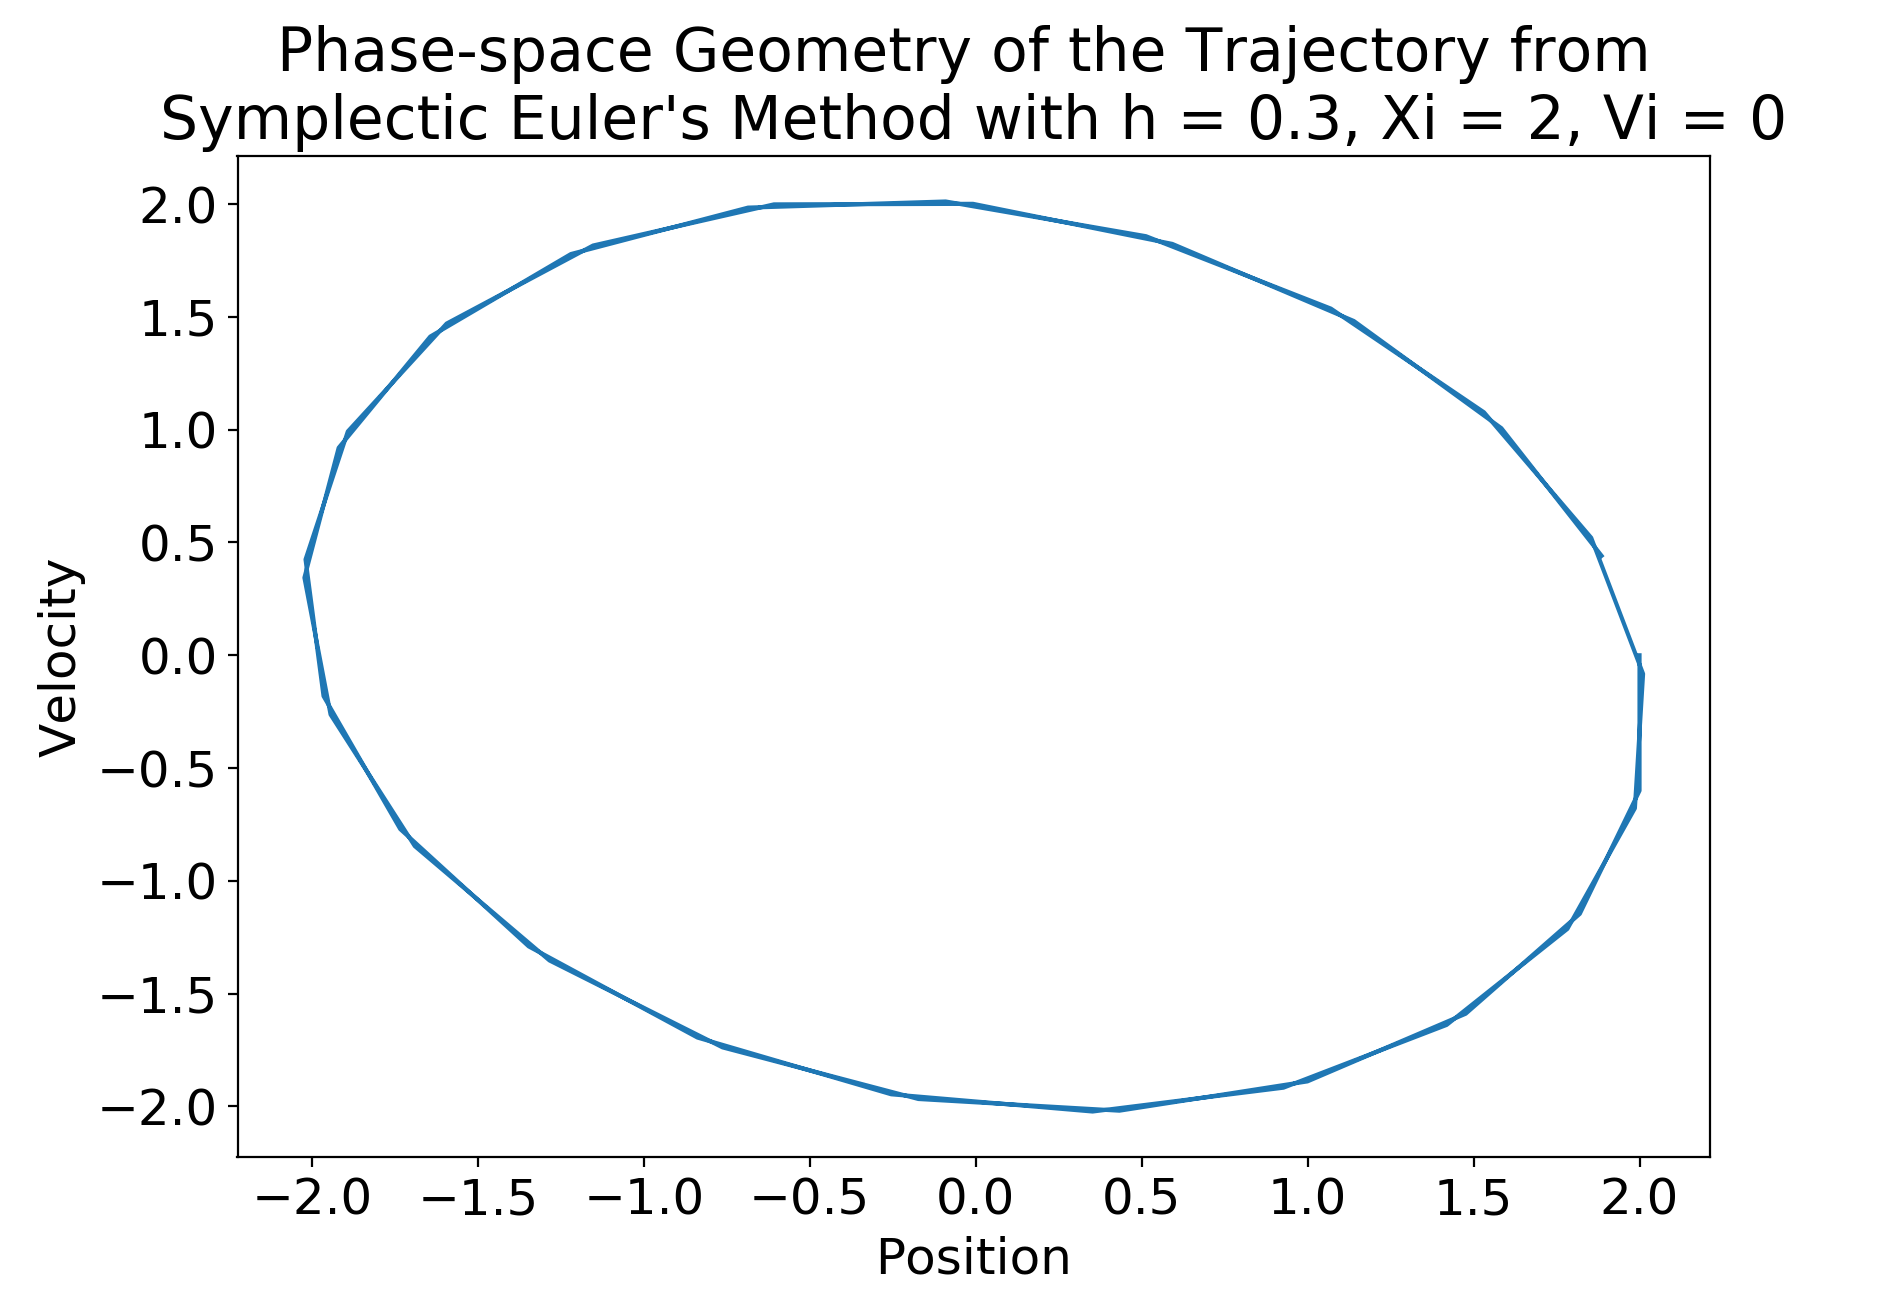
\includegraphics[width=1\linewidth]{PSGeoSym3.png}
\end{subfigure}
\begin{subfigure}{.3\textwidth}
  \centering
  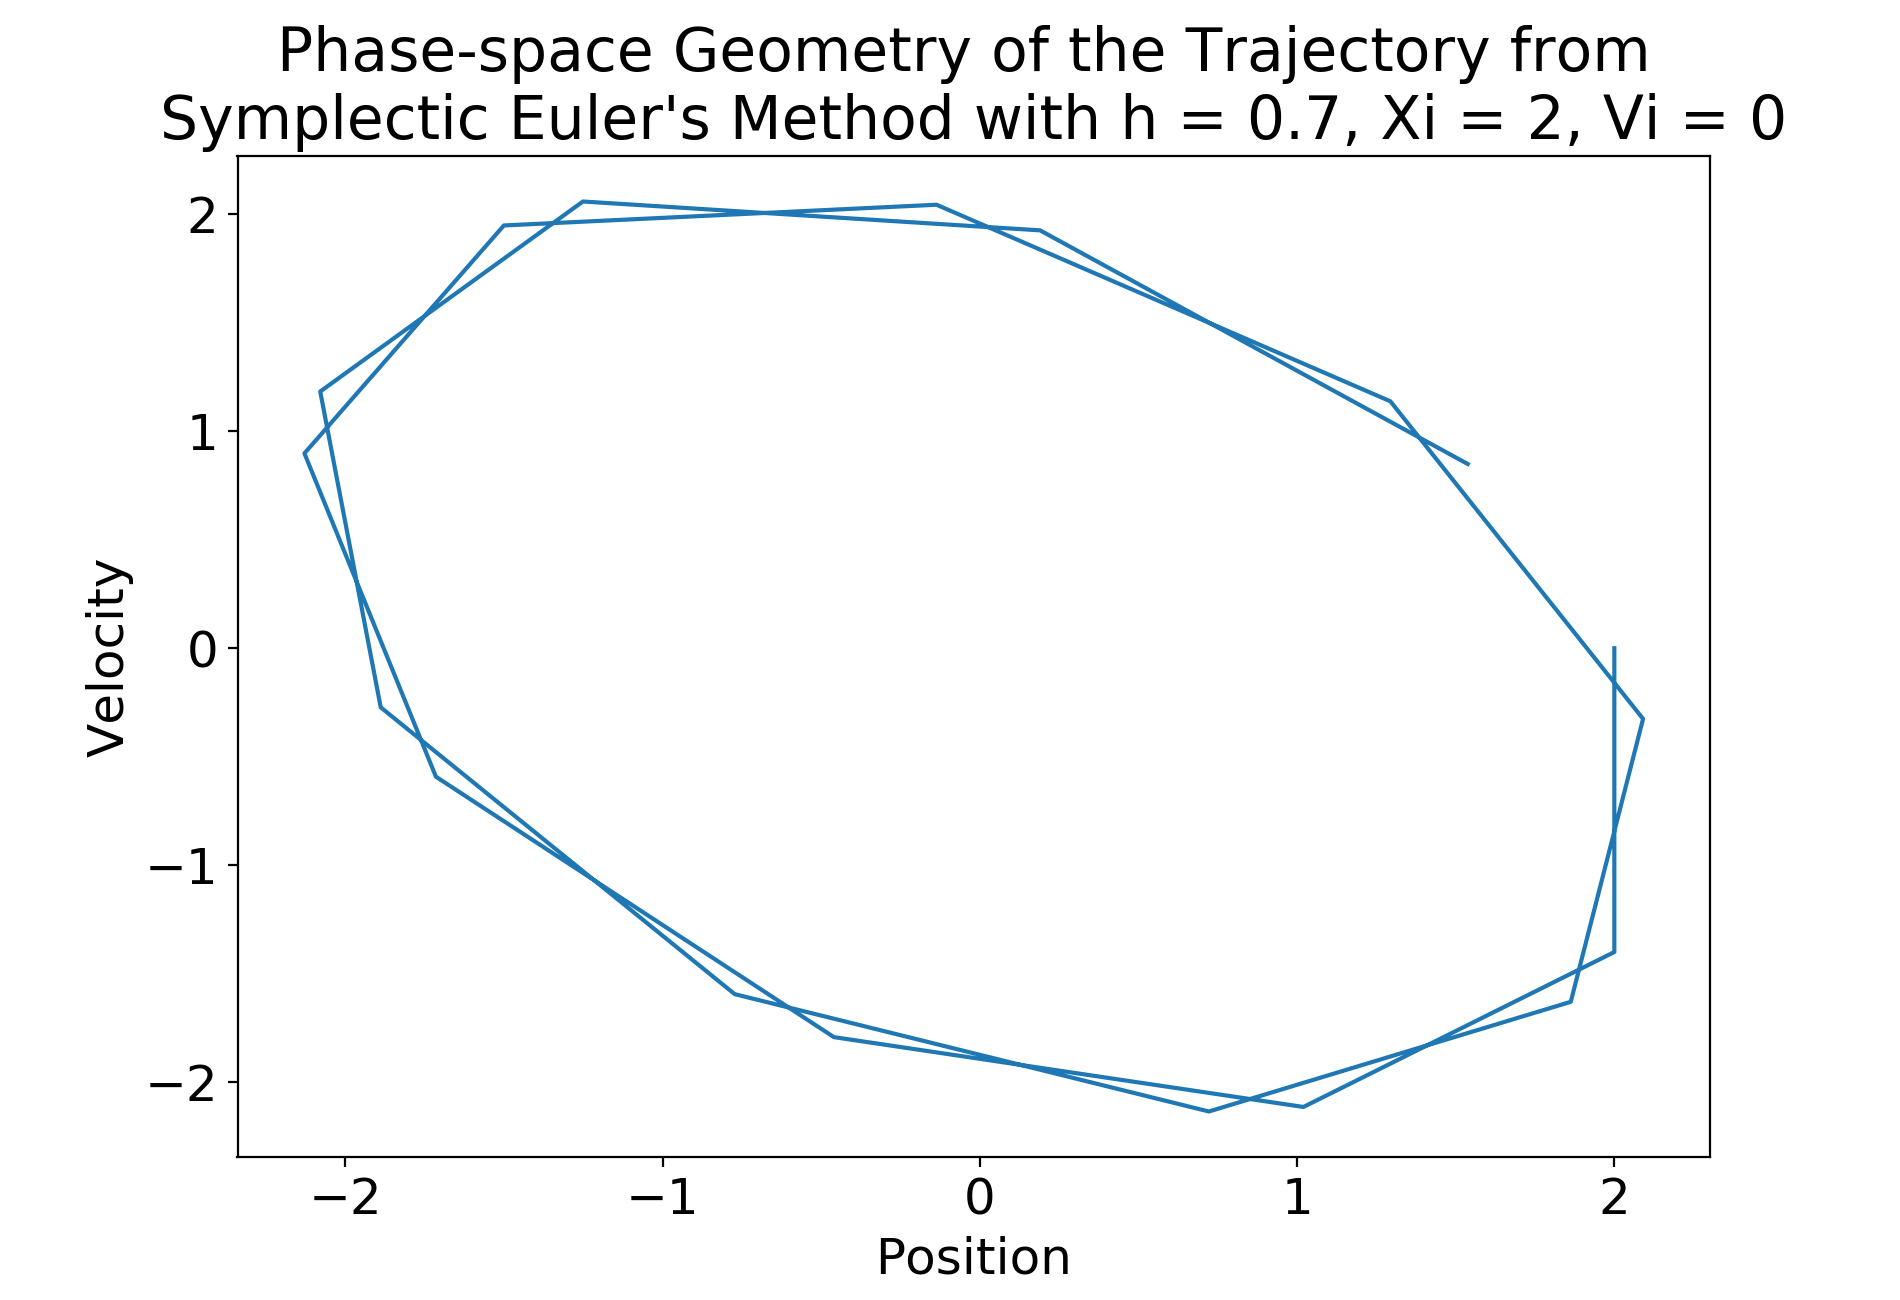
\includegraphics[width=1\linewidth]{PSGeoSym7.png}
\end{subfigure}
\caption{Evolution of a Spring's Position and Velocity as Given by the Symplectic Euler's Method}
\end{figure}
\end{problem}

\newpage
\begin{problem} {8}
The phase-space of geometry of the spring as modelled using the symplectic Euler's method suggests an fairly regular energy. This conclusion is confirmed by the plot of its energy as a function of time, which appears to vary cyclically within a relatively small range. Furthermore, these cycles correspond in number to the number of oscillations in the spring, so energy is remaining constant from oscillation to oscillation. As a result, the energy of the system should not change dramatically over the course of a few many oscillations, as it does with the explicit and implicit Euler's method.
\begin{figure} [h]
\centering
    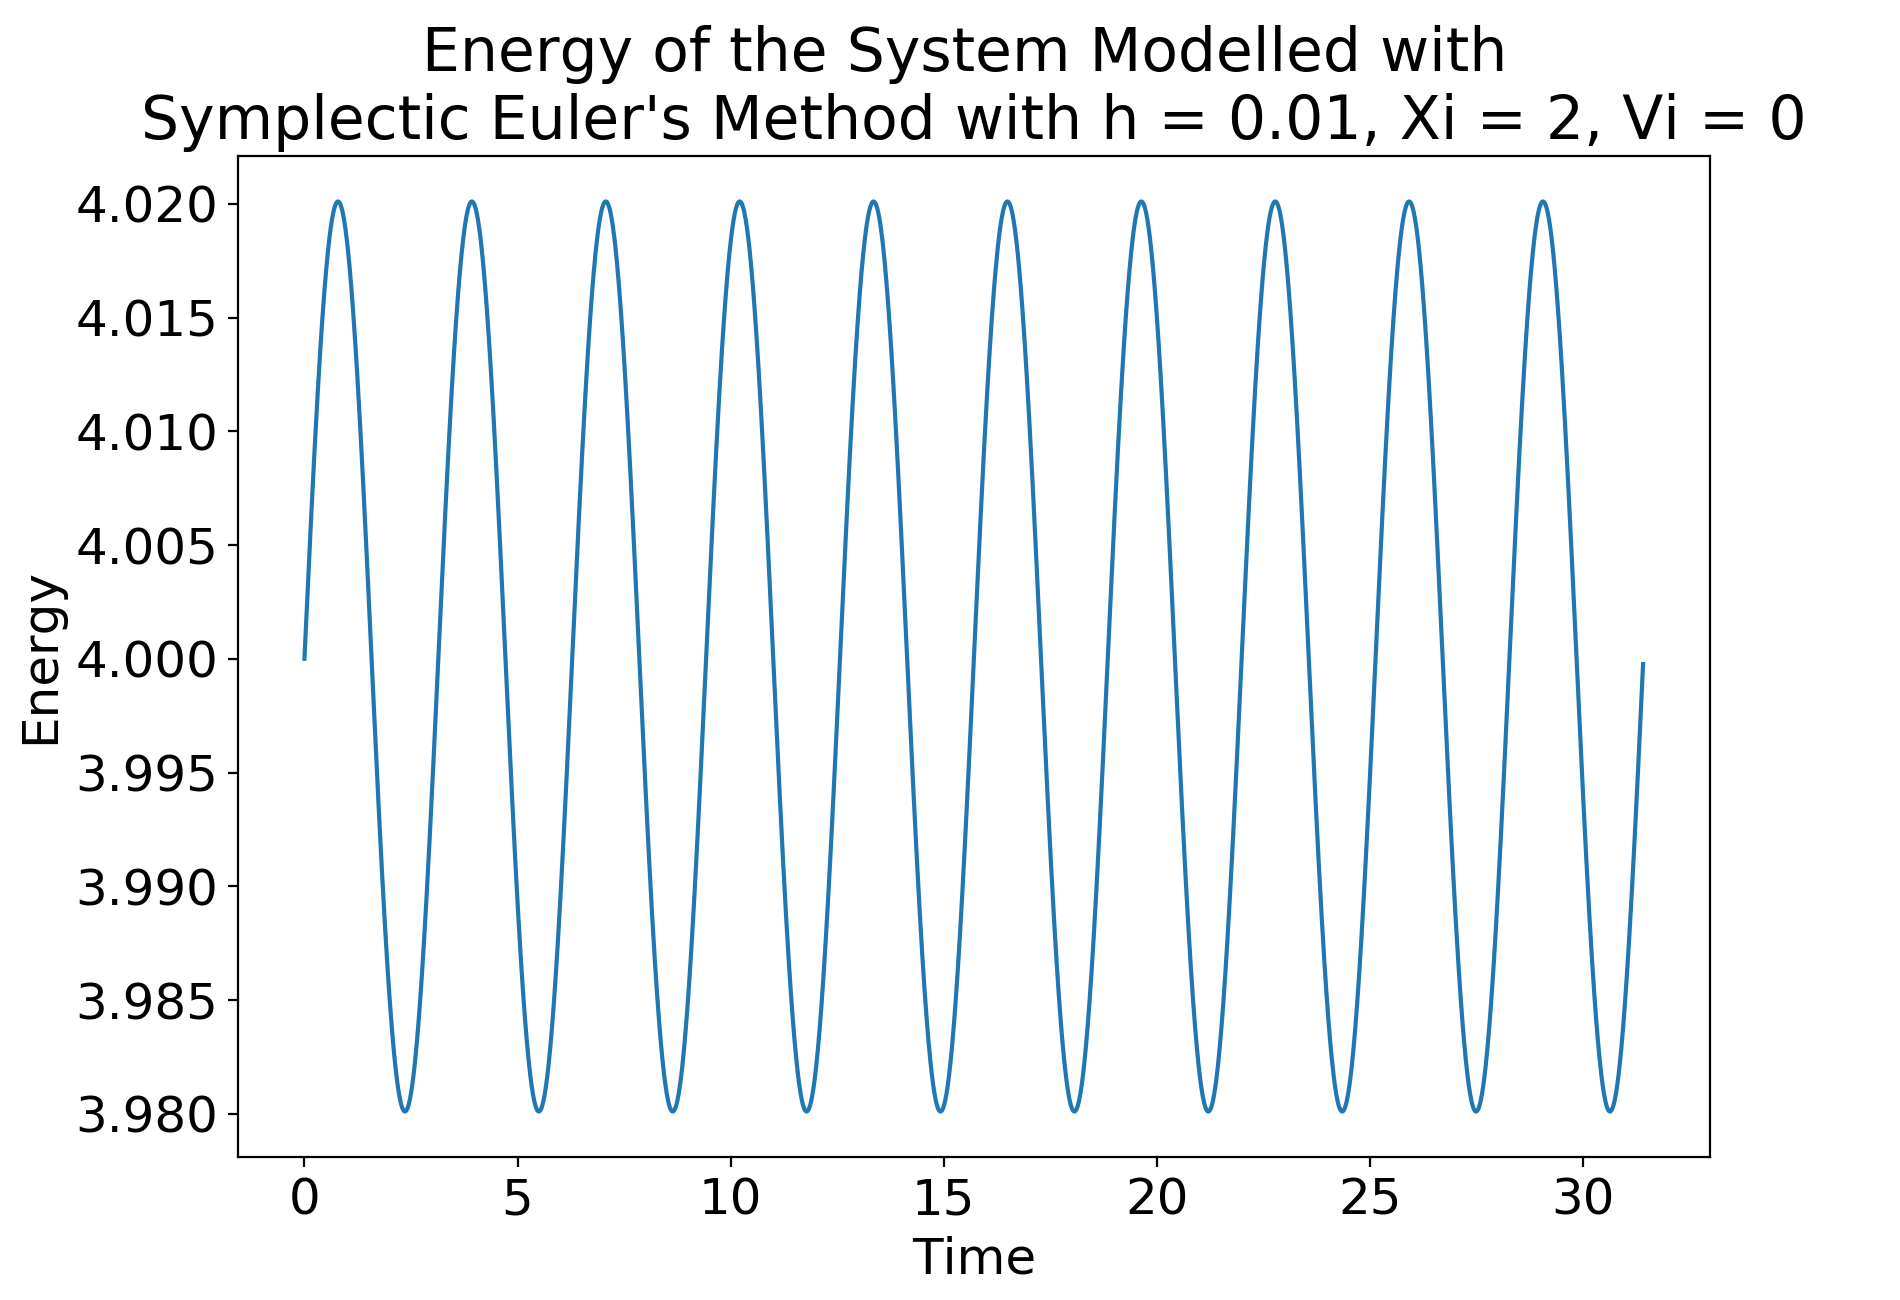
\includegraphics[width=.7\linewidth]{NrgSym.png}
\centering
    \caption{Energy of a Spring Modelled by Symplectic Euler's Rule for 10 Oscillations}
\end{figure}
\end{problem}

\end{document}